\documentclass[12pt,english]{article}\usepackage[]{graphicx}\usepackage[table]{xcolor}
% maxwidth is the original width if it is less than linewidth
% otherwise use linewidth (to make sure the graphics do not exceed the margin)
\makeatletter
\def\maxwidth{ %
  \ifdim\Gin@nat@width>\linewidth
    \linewidth
  \else
    \Gin@nat@width
  \fi
}
\makeatother

\definecolor{fgcolor}{rgb}{0.345, 0.345, 0.345}
\newcommand{\hlnum}[1]{\textcolor[rgb]{0.686,0.059,0.569}{#1}}%
\newcommand{\hlsng}[1]{\textcolor[rgb]{0.192,0.494,0.8}{#1}}%
\newcommand{\hlcom}[1]{\textcolor[rgb]{0.678,0.584,0.686}{\textit{#1}}}%
\newcommand{\hlopt}[1]{\textcolor[rgb]{0,0,0}{#1}}%
\newcommand{\hldef}[1]{\textcolor[rgb]{0.345,0.345,0.345}{#1}}%
\newcommand{\hlkwa}[1]{\textcolor[rgb]{0.161,0.373,0.58}{\textbf{#1}}}%
\newcommand{\hlkwb}[1]{\textcolor[rgb]{0.69,0.353,0.396}{#1}}%
\newcommand{\hlkwc}[1]{\textcolor[rgb]{0.333,0.667,0.333}{#1}}%
\newcommand{\hlkwd}[1]{\textcolor[rgb]{0.737,0.353,0.396}{\textbf{#1}}}%
\let\hlipl\hlkwb

\usepackage{framed}
\makeatletter
\newenvironment{kframe}{%
 \def\at@end@of@kframe{}%
 \ifinner\ifhmode%
  \def\at@end@of@kframe{\end{minipage}}%
  \begin{minipage}{\columnwidth}%
 \fi\fi%
 \def\FrameCommand##1{\hskip\@totalleftmargin \hskip-\fboxsep
 \colorbox{shadecolor}{##1}\hskip-\fboxsep
     % There is no \\@totalrightmargin, so:
     \hskip-\linewidth \hskip-\@totalleftmargin \hskip\columnwidth}%
 \MakeFramed {\advance\hsize-\width
   \@totalleftmargin\z@ \linewidth\hsize
   \@setminipage}}%
 {\par\unskip\endMakeFramed%
 \at@end@of@kframe}
\makeatother

\definecolor{shadecolor}{rgb}{.97, .97, .97}
\definecolor{messagecolor}{rgb}{0, 0, 0}
\definecolor{warningcolor}{rgb}{1, 0, 1}
\definecolor{errorcolor}{rgb}{1, 0, 0}
\newenvironment{knitrout}{}{} % an empty environment to be redefined in TeX

\usepackage{alltt}
\usepackage{tcolorbox}
\usepackage{graphics, color}
\usepackage{natbib} % \usepackage{ragged2e}
\usepackage{amssymb}
\usepackage{amsmath}
\usepackage{graphicx}
\usepackage{setspace}
\usepackage{booktabs}% http://ctan.org/pkg/booktabs
\newcommand{\tabitem}{~~\llap{\textbullet}~~}
\usepackage{BOONDOX-cal}
\usepackage[colorlinks=false, linkcolor = black]{hyperref} % draft turns off -- hyperlinks\usepackage[draft, colorlinks=false, linkcolor = black]{hyperref}
\usepackage{footnote}
\usepackage{csquotes}
\usepackage{pdflscape}
\usepackage{fullpage} % \usepackage{threeparttable}
\usepackage{float}
\usepackage{array}% http://ctan.org/pkg/array


\usepackage[margin=1in]{geometry}

\hypersetup{
    colorlinks,
    linkcolor={red!50!black},
    citecolor={blue!50!black},
    urlcolor={blue!80!black}
}


\usepackage{exercise}
\newcommand{\mydate}{Updated: }
\renewcommand{\ExerciseName}{Example}

\usepackage{caption}
\usepackage[table]{xcolor}


\usepackage[protrusion=true,expansion=true]{microtype}	


% --------------------------------------------------------------------
% Definitions (do not change this)
% --------------------------------------------------------------------
\newcommand{\HRule}[1]{\rule{\linewidth}{#1}} 	% Horizontal rule

\makeatletter							% Title
\def\printtitle{%						
    {\centering \@title\par}}
\makeatother									

\makeatletter							% Author
\def\printauthor{%					
    {\centering \large \@author}}				
\makeatother							

% --------------------------------------------------------------------
% Metadata (Change this)
% --------------------------------------------------------------------
\title{	\normalsize \textsc{} 	% Subtitle
		 	\\[0.2cm]								% 2cm spacing
			\HRule{0.5pt} \\						% Upper rule
			\LARGE \textbf{\uppercase{ANOVA Frameworks Using \textbf{R}}}	% Title
			\HRule{0.5pt} \\ [1.5cm]
			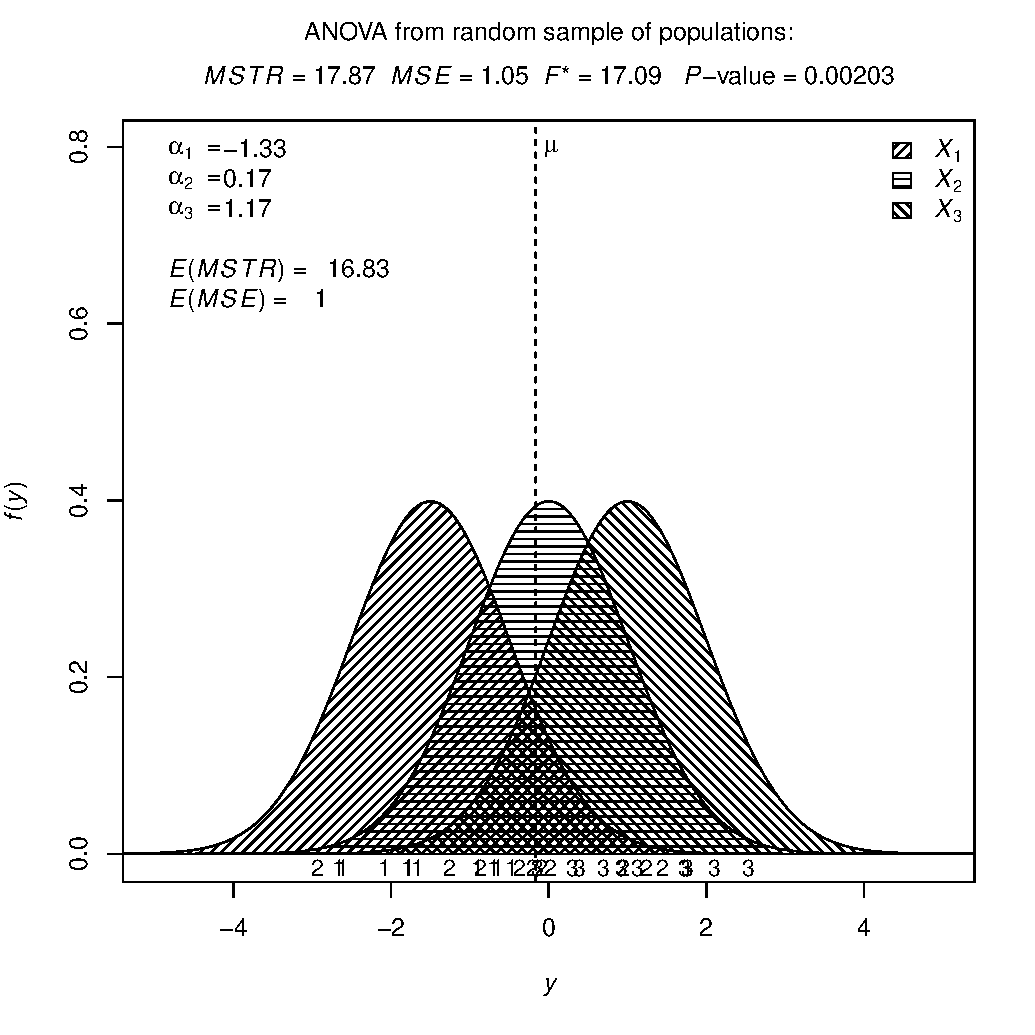
\includegraphics[width=0.95\textwidth]{cover.pdf}\\ [0.5cm]% Lower rule + 0.5cm spacing
					% Todays date
		}

\author{
		Ken Aho\\
		\begin{center}
		\normalsize{\mydate \today}	
		\end{center}
}
\IfFileExists{upquote.sty}{\usepackage{upquote}}{}
\begin{document}




\thispagestyle{empty}		% Remove page numbering on this page

\printtitle					% Print the title data as defined above
  	\vfill
\printauthor				% Print the author data as defined above
\newpage
% ------------------------------------------------------------------------------
% Begin document
% ------------------------------------------------------------------------------
\setcounter{page}{1}		% Set page numbering to begin on this page




\thispagestyle{empty}
%\afterpage{\null\newpage}
\setcounter{page}{1}

\tableofcontents
\vspace*{\fill}
\newpage

\section{Inference to One Population Mean}
\subsection{One sample $z$-test}

\noindent \textbf{H$_0$:} $\mu = \mu_0$, where $\mu_0$ is a stipulated null value. Directional alternative hypotheses are possible.

\vspace{0.1in}
\noindent \textbf{Assumptions:} Underlying distribution is normal with mean $\mu$, and known variance, $\sigma^2$.

\vspace{0.2in}
\noindent \textbf{Robust Alternatives:}
\begin{small}
\begin{itemize}
\item Kolmogorov-Smirnov test of the equality of continuous, one-dimensional, probability distributions \citep{kolmogorov1933, smirnov1948}, \textbf{R:} \texttt{ks.test()}
\vspace{-.1in}
\item Many others \citep[see][]{wilcox2012, hollander2013}.
\end{itemize}
\end{small}
\vspace{0.1in}
\par\noindent\rule{.9\textwidth}{0.4pt}
\begin{tcolorbox}[colback=yellow!50!red!25!white,colbacktitle=yellow!50!red,colframe=black!75!white,title=\textbf{R:} One Sample $z$-Test]

\textbf{Framework:}\\
\vspace{-.2in}
\begin{knitrout}
\definecolor{shadecolor}{rgb}{0.969, 0.969, 0.969}\color{fgcolor}\begin{kframe}
\begin{alltt}
\hlkwd{library}\hldef{(asbio)}
\hlkwd{one.sample.z}\hldef{(Y)}
\end{alltt}
\end{kframe}
\end{knitrout}
\vspace{-.1in}

\texttt{Y} = response variable.
\vspace{0.1in}
%\par\noindent\rule{.9\textwidth}{0.4pt}

\textbf{Example:} From \citep[][pp 206-207]{aho2014}.  \citet{port2000} found that for males 45-54 years of age systolic  blood pressure was normally distributed with $\mu= 131$ mmHg (millimeters of mercury), and $\sigma = 12$ mmHg.  A medical administrator at a state university examines the records of 85 male faculty members in this age group and finds that $\bar{x} = 128$ mmHg.   The administrator wondered if the blood pressure of faculty members at this university differed from that of the overall population of males 45-54 years of age.
\vspace{-.1in}
\begin{knitrout}
\definecolor{shadecolor}{rgb}{0.969, 0.969, 0.969}\color{fgcolor}\begin{kframe}
\begin{alltt}
\hlkwd{library}\hldef{(asbio)}
\hlkwd{one.sample.z}\hldef{(}\hlkwc{null.mu} \hldef{=} \hlnum{131}\hldef{,} \hlkwc{xbar} \hldef{=} \hlnum{128}\hldef{,} \hlkwc{sigma} \hldef{=} \hlnum{12}\hldef{,} \hlkwc{n} \hldef{=} \hlnum{85}\hldef{,}
             \hlkwc{alternative} \hldef{=} \hlsng{"two.sided"}\hldef{)}
\end{alltt}
\end{kframe}
\end{knitrout}
\end{tcolorbox}

\par\noindent\rule{.9\textwidth}{0.4pt}


\subsection{One sample $t$-test}

\noindent \textbf{H$_0$:} $\mu = \mu_0$, where $\mu_0$ is a stipulated null value. Directional alternative hypotheses are possible.

\vspace{0.1in}
\noindent \textbf{Assumptions:} Underlying distribution is normal with mean $\mu$.
\vspace{0.1in}

\noindent \textbf{Robust Alternatives:}
\begin{small}
\begin{itemize}
\item Kolmogorov-Smirnov test of the equality of continuous, one-dimensional probability distributions \citep{kolmogorov1933, smirnov1948}, \textbf{R:} \texttt{ks.test()}\vspace{-.1in}
\item Many others \citep[see][]{wilcox2012, hollander2013}.
\end{itemize}
\end{small}

\vspace{0.2in}
%\par\noindent\rule{.9\textwidth}{0.4pt}
\begin{tcolorbox}[colback=yellow!50!red!25!white,colbacktitle=yellow!50!red,colframe=black!75!white,title=\textbf{R:} One Sample $t$-Test]


\textbf{Framework:}\\
\vspace{-.2in}
\begin{knitrout}
\definecolor{shadecolor}{rgb}{0.969, 0.969, 0.969}\color{fgcolor}\begin{kframe}
\begin{alltt}
\hlkwd{library}\hldef{(asbio)}
\hlkwd{one.sample.t}\hldef{(Y)}
\end{alltt}
\end{kframe}
\end{knitrout}
\vspace{-.1in}

\texttt{Y} = response variable.
\vspace{0.1in}
\par\noindent\rule{.9\textwidth}{0.4pt}

\textbf{Example:} From \citep[][pp 206-207]{aho2014} see text details for one sample $z$-test above.
\vspace{-.1in}
\begin{knitrout}
\definecolor{shadecolor}{rgb}{0.969, 0.969, 0.969}\color{fgcolor}\begin{kframe}
\begin{alltt}
\hlkwd{library}\hldef{(asbio)}
\hlkwd{one.sample.t}\hldef{(}\hlkwc{null.mu} \hldef{=} \hlnum{131}\hldef{,} \hlkwc{xbar} \hldef{=} \hlnum{128}\hldef{,} \hlkwc{s} \hldef{=} \hlnum{12}\hldef{,} \hlkwc{n} \hldef{=} \hlnum{85}\hldef{,}
             \hlkwc{alternative} \hldef{=} \hlsng{"two.sided"}\hldef{)}
\end{alltt}
\end{kframe}
\end{knitrout}
\end{tcolorbox}
\par\noindent\rule{.9\textwidth}{0.4pt}


\newpage





\section{Two Groups}
\subsection{Assumed Homoscedasticity -- Pooled Variance $t$-Test}
\textbf{Model:} \[Y_{ij} = \mu + \alpha_i + \varepsilon_{ij} \hspace{0.2in} \left\{
                \begin{array}{ll}
                  i = 1,2\\
                  j = 1,2,\dots,n_i\\
                  \end{array}
              \right.\]

\noindent where $Y_{ij}$ is the \textit{j}th response for the \textit{i}th factor level, $\mu$ is the true grand mean, $\alpha_i$ is the \textit{i}th factor level effect, e.g., $\alpha_i = \mu_i - \mu$ (where $\mu_i$ is the true \textit{i}th factor level mean), and $\varepsilon_{ij}$ is the \textit{j}th error in the \textit{i}th factor level. \\
\vspace{0.05in}

\noindent \textbf{H$_0$:} $\mu_1 - \mu_2 = D_0$, where $D_0$ is a stipulated null difference, generally taken to be 0. Directional alternative hypotheses are possible.

\vspace{0.1in}
\noindent \textbf{Assumptions:} 
$\varepsilon_{ij} \sim N(0, \sigma^2)$.
\vspace{0.1in}

\noindent \textbf{Robust Alternatives:}

\begin{small}
\begin{itemize}
\item Wilcoxon rank sum test \citep{wilcoxon1945}, robust to outliers and non-normal errors, \textbf{R:} \texttt{wilcox.test(paired = F)}\vspace{-.1in}
\item Welch test \citep{welch1951}, robust to heteroscedasticity but requires normal errors, \textbf{R:} \texttt{oneway.test}, \texttt{t.test(var.equal = F)}\vspace{-.1in}
\item Brunner-Dette-Munk test \citep{brunner1997}, robust to outliers, non-normal errors and heteroscedasticity, \textbf{R:} \texttt{asbio::BDM.test}\vspace{-.1in}
\item Permutation tests \citep[see][]{manly2006}, \textbf{R:} \texttt{asbio::MC.test}
\item Many others \citep[see][]{wilcox2012, hollander2013}.
\end{itemize}
\end{small}
\vspace{0.1in}
%\par\noindent\rule{.9\textwidth}{0.4pt}
\begin{tcolorbox}[colback=yellow!50!red!25!white,colbacktitle=yellow!50!red,colframe=black!75!white,title=\textbf{R:} Pooled Variance $t$-Test]


\textbf{Framework:}\\
\vspace{-.2in}
\begin{knitrout}
\definecolor{shadecolor}{rgb}{0.969, 0.969, 0.969}\color{fgcolor}\begin{kframe}
\begin{alltt}
\hlkwd{t.test}\hldef{(Y} \hlopt{~} \hldef{A,} \hlkwc{var.equal} \hldef{= T)}
\end{alltt}
\end{kframe}
\end{knitrout}
\vspace{-.1in}
or
\vspace{-.1in}
\begin{knitrout}
\definecolor{shadecolor}{rgb}{0.969, 0.969, 0.969}\color{fgcolor}\begin{kframe}
\begin{alltt}
\hlkwd{t.test}\hldef{(X1, X2,} \hlkwc{var.equal} \hldef{= T)}
\end{alltt}
\end{kframe}
\end{knitrout}
\texttt{Y} = response variable, \texttt{A} = a factor with two levels, \texttt{X1} = observations from first level, \texttt{X2} = observations from second level.
\vspace{0.1in}
\par\noindent\rule{.9\textwidth}{0.4pt}

\textbf{Example:} From \citep[][pp 215-217]{aho2014}.  \citet{monteith2009} examined the maternal life history characteristics of white-tailed deer (\textit{Odocoileus virginianus}) originating from the Black Hills in southwestern South Dakota and from eastern South Dakota. Because litter size and dam size affects offspring weight the investigators used proportional birth mass (dam mass/total litter mass) as a measure of reproductive investment by deer.
\vspace{-.1in}
\begin{knitrout}
\definecolor{shadecolor}{rgb}{0.969, 0.969, 0.969}\color{fgcolor}\begin{kframe}
\begin{alltt}
\hlkwd{library}\hldef{(asbio);} \hlkwd{data}\hldef{(deer)}
\hlkwd{with}\hldef{(deer,} \hlkwd{t.test}\hldef{(Prop.mass} \hlopt{~} \hldef{Region,} \hlkwc{var.equal} \hldef{= T))}
\end{alltt}
\end{kframe}
\end{knitrout}
\end{tcolorbox}
\par\noindent\rule{.9\textwidth}{0.4pt}

\subsection{Heteroscedasticity -- Welch $t$-Test}
\textbf{Model:} \[Y_{ij} = \mu + \alpha_i + \varepsilon_{ij} \hspace{0.2in} \left\{
                \begin{array}{ll}
                  i = 1,2\\
                  j = 1,2,\dots,n_i\\
                  \end{array}
              \right.\]

\noindent where $Y_{ij}$ is the \textit{j}th response for the \textit{i}th factor level, $\mu$ is the true grand mean, $\alpha_i$ is the \textit{i}th factor level effect, e.g., $\alpha_i = \mu_i - \mu$ (where $\mu_i$ is the true \textit{i}th factor level mean), and $\varepsilon_{ij}$ is the \textit{j}th error in the \textit{i}th factor level. \\
\vspace{0.05in}

\noindent \textbf{H$_0$:} $\mu_1 - \mu_2 = D_0$, where $D_0$ is a stipulated null difference, generally taken to be 0. Directional alternative hypotheses are possible.

\vspace{0.1in}

\noindent \textbf{Assumptions:} $\varepsilon_{ij}$ are normal, homoscedasticity not required.
\vspace{0.1in}

\noindent \textbf{Robust Alternatives:}
\begin{small}
\begin{itemize}
\item Brunner-Dette-Munk test \citep{brunner1997}, robust to outliers, non-normal errors and heteroscedasticity, \textbf{R:} \texttt{asbio::BDM.test}\vspace{-.1in}
\end{itemize}
\end{small}
\vspace{0.1in}
%\par\noindent\rule{.9\textwidth}{0.4pt}
\begin{tcolorbox}[colback=yellow!50!red!25!white,colbacktitle=yellow!50!red,colframe=black!75!white,title=\textbf{R:} Welch $t$-Test]


\textbf{Framework:}\\
\vspace{-.2in}
\begin{knitrout}
\definecolor{shadecolor}{rgb}{0.969, 0.969, 0.969}\color{fgcolor}\begin{kframe}
\begin{alltt}
\hlkwd{t.test}\hldef{(Y} \hlopt{~} \hldef{A)}\hlcom{# var.equal = F is the default value}
\end{alltt}
\end{kframe}
\end{knitrout}
\vspace{-.1in}
or
\vspace{-.1in}
\begin{knitrout}
\definecolor{shadecolor}{rgb}{0.969, 0.969, 0.969}\color{fgcolor}\begin{kframe}
\begin{alltt}
\hlkwd{t.test}\hldef{(X1, X2)}
\end{alltt}
\end{kframe}
\end{knitrout}
\texttt{Y} = response variable, \texttt{A} = a factor with two levels, \texttt{X1} = observations from first level, \texttt{X2} = observations from second level.
\vspace{0.1in}
\par\noindent\rule{.9\textwidth}{0.4pt}

\textbf{Example:} From \citep[][pg 217-218]{aho2014}.  \citet{vallbona1997} tested whether chronic pain experienced by post-polio patients could be treated with magnetic fields applied directly to pain trigger points. The investigators identified fifty subjects who not only had post-polio syndrome, but who also experienced muscular or arthritic pain. Magnets were applied to pain trigger points in 29 randomly selected subjects, and in the other 21 a placebo was applied. The patients were asked to subjectively rate pain on a scale from one to ten before and after application of the magnet or placebo.
\vspace{-.1in}
\begin{knitrout}
\definecolor{shadecolor}{rgb}{0.969, 0.969, 0.969}\color{fgcolor}\begin{kframe}
\begin{alltt}
\hlkwd{library}\hldef{(asbio);} \hlkwd{data}\hldef{(magnets)}
\hlkwd{with}\hldef{(magnets,} \hlkwd{t.test}\hldef{(Score_1} \hlopt{-} \hldef{Score_2} \hlopt{~} \hldef{Active,}
                     \hlkwc{alternative} \hldef{=} \hlsng{"greater"}\hldef{))}
\end{alltt}
\end{kframe}
\end{knitrout}
\end{tcolorbox}
\par\noindent\rule{.9\textwidth}{0.4pt}

\subsection{Paired Design -- Paired $t$-Test}

\noindent \textbf{Model:} \[Y_{ij} = \mu + \alpha_i + \beta_j + \varepsilon_{ij}  \hspace{0.2in} \left\{
                \begin{array}{ll}
                  i = 1,2\\
                  j = 1,2\\
              \end{array}
              \right.\]

\noindent where $Y_{ij}$ is the response for the \textit{i}th factor level in the $j$th pairing, $\mu$ is the true grand mean, $\alpha_i$ is the \textit{i}th factor level effect, $\beta_j$ is the $j$th pairing effect, and $\varepsilon_{ij}$ is the \textit{j}th block error in the \textit{i}th factor level. \\
\vspace{0.05in}

\noindent \textbf{H$_0$:} $\mu_D = D_0$, where $\mu_D$ is the true mean of paired differences, and $D_0$ is a stipulated null difference, generally taken to be 0.  Directional alternative hypotheses are possible.

\vspace{0.1in}
\noindent \textbf{Assumptions:} $\varepsilon_{ij} \sim N(0, \sigma^2)$; all $(\alpha\beta)_{ij} = 0$
\vspace{0.1in}

\noindent \textbf{Robust Alternatives:}
\begin{small}
\begin{itemize}
\item Wilcoxon sign rank test \citep{wilcoxon1945}, robust to outliers and non-normal errors, \textbf{R:} \texttt{wilcox.test(paired = T)}
\end{itemize}
\end{small}
\vspace{0.1in}

\begin{tcolorbox}[colback=yellow!50!red!25!white,colbacktitle=yellow!50!red,colframe=black!75!white,title=\textbf{R:} Paired $t$-Test]
\textbf{Framework:}\\
\vspace{-.2in}
\begin{knitrout}
\definecolor{shadecolor}{rgb}{0.969, 0.969, 0.969}\color{fgcolor}\begin{kframe}
\begin{alltt}
\hlkwd{t.test}\hldef{(Y} \hlopt{~} \hldef{A,} \hlkwc{paired} \hldef{= T)}
\end{alltt}
\end{kframe}
\end{knitrout}
\vspace{-.1in}
or
\vspace{-.1in}
\begin{knitrout}
\definecolor{shadecolor}{rgb}{0.969, 0.969, 0.969}\color{fgcolor}\begin{kframe}
\begin{alltt}
\hlkwd{t.test}\hldef{(X1, X2,} \hlkwc{paired} \hldef{= T)}
\end{alltt}
\end{kframe}
\end{knitrout}
\texttt{Y} = response variable, \texttt{A} = a factor with two levels, \texttt{X1} = observations from first level, \texttt{X2} = observations from second level.
\vspace{0.1in}
\par\noindent\rule{.9\textwidth}{0.4pt}

\textbf{Example:} From \citep{aho2014}.  To control for confounding variables, \citet{suddath1990} examined 15 pairs of monozygotic twins where one twin was schizophrenic and the other was not. Twins were located from an intensive search throughout the United States and Canada. The authors used magnetic resonance imaging to measure brain volume of particular regions in the twin's brains.
\vspace{-.1in}
\begin{knitrout}
\definecolor{shadecolor}{rgb}{0.969, 0.969, 0.969}\color{fgcolor}\begin{kframe}
\begin{alltt}
\hlkwd{library}\hldef{(asbio);} \hlkwd{data}\hldef{(sc.twin)}
\hlkwd{with}\hldef{(sc.twin,} \hlkwd{t.test}\hldef{(unaffected, affected,} \hlkwc{paired} \hldef{= T))}
\end{alltt}
\end{kframe}
\end{knitrout}
\end{tcolorbox}
\par\noindent\rule{.9\textwidth}{0.4pt}
\newpage



\section{Completely Randomized Design, One Factor, $\geq 2$ Levels}
In a \textit{completely randomized design} (CRD), experimental units are each randomly assigned to factor levels without constraints like blocking.

%%%%%%%%%%%%%%%%%%%%%%%%%%%%%%%%%%%%%%%%%%%%%%%%%%%%%%%%%%%%%%%%%%%%%%%%%%%%%%%%%%%%%%%%%%%%%%%%%%%%%%%%%%%%%%%%
\subsection{One Way ANOVA - Fixed Effects}

\textbf{Model:} \[Y_{ij} = \mu + \alpha_i + \varepsilon_{ij} \hspace{0.2in} \left\{
                \begin{array}{ll}
                  i = 1,2,\dots,a\\
                  j = 1,2,\dots,n\\
                  \end{array}
              \right.\]



\noindent where $Y_{ij}$ is the \textit{j}th response for the \textit{i}th factor level, $\mu$ is the true grand mean, $\alpha_i$ is the \textit{i}th factor level effect, e.g., $\alpha_i = \mu_i - \mu$ (where $\mu_i$ is the true \textit{i}th factor level mean), and $\varepsilon_{ij}$ is the \textit{j}th error in the \textit{i}th factor level. \\
\vspace{0.05in}

\noindent \textbf{H$_0$:} $\mu_1 = \mu_2 = \dots = \mu_a$.

\vspace{0.1in}
\noindent \textbf{Assumptions:} $\varepsilon_{ij} \sim N(0, \sigma^2)$.
\vspace{0.1in}

\noindent \textbf{Robust Alternatives:}
\begin{small}
\begin{itemize}
\item Kruskal-Wallis test \citep{kruskal1952}, robust to outliers and non-normal errors, \textbf{R:} \texttt{kruskal.test}\vspace{-.1in}
\item Welch test \citep{welch1951}, robust to heteroscedasticity but requires normal errors, \textbf{R:} \texttt{oneway.test}\vspace{-.1in}
\item Brunner-Dette-Munk test \citep{brunner1997}, robust to outliers, non-normal errors and heteroscedasticity, \textbf{R:} \texttt{asbio::BDM.test}\vspace{-.1in}
\item Permutation tests \citep[see][]{manly2006}, \textbf{R:} \texttt{asbio::MC.test}
\end{itemize}
\end{small}
\vspace{0.1in}
%\par\noindent\rule{.9\textwidth}{0.4pt}
\begin{tcolorbox}[colback=yellow!50!red!25!white,colbacktitle=yellow!50!red,colframe=black!75!white,title=\textbf{R:} One Way ANOVA - Fixed Effects]

\textbf{Framework:}\\
\vspace{-.2in}
\begin{knitrout}
\definecolor{shadecolor}{rgb}{0.969, 0.969, 0.969}\color{fgcolor}\begin{kframe}
\begin{alltt}
\hlkwd{anova}\hldef{(}\hlkwd{lm}\hldef{(Y} \hlopt{~} \hldef{A))}
\end{alltt}
\end{kframe}
\end{knitrout}
\vspace{-.1in}
or
\vspace{-.1in}
\begin{knitrout}
\definecolor{shadecolor}{rgb}{0.969, 0.969, 0.969}\color{fgcolor}\begin{kframe}
\begin{alltt}
\hlkwd{aov}\hldef{(Y} \hlopt{~} \hldef{A)}
\end{alltt}
\end{kframe}
\end{knitrout}
\texttt{Y} = response variable, \texttt{A} = predictor, i.e., a factor.
\vspace{0.1in}
\par\noindent\rule{.9\textwidth}{0.4pt}

\textbf{Example:} From \citep[][pg 52]{litt2002}.  Five specimens of each of five brands of a synthetic wood veneer material were subjected to a friction test.
\vspace{-.1in}
\begin{knitrout}
\definecolor{shadecolor}{rgb}{0.969, 0.969, 0.969}\color{fgcolor}\begin{kframe}
\begin{alltt}
\hlkwd{library}\hldef{(asbio);} \hlkwd{data}\hldef{(veneer)}
\hlkwd{anova}\hldef{(}\hlkwd{lm}\hldef{(wear} \hlopt{~} \hldef{brand,} \hlkwc{data} \hldef{= veneer))}
\end{alltt}
\end{kframe}
\end{knitrout}
\end{tcolorbox}
%%%%%%%%%%%%%%%%%%%%%%%%%%%%%%%%%%%%%%%%%%%%%%%%%%%%%%%%%%%%%%%%%%%%%%%%%%%%%%%%%%%%%%%%%%%%%%%%%%%%%%%%%%%%%
\par\noindent\rule{.9\textwidth}{0.4pt}

\subsection{One Way ANOVA - Random Effects}
% \noindent\textbf{A Word on Random Effects in R:}\\
 \noindent As noted in \citet{aho2014}:

\begin{quote}
\dots random factor levels have two characteristics: 1) they can be considered a sample from a population of factor levels, and 2) they will not be informative.  Because they are non-informative, comparisons among random factor levels means are of little interest. Instead, investigators will generally be interested in making inference to the true variance of the distribution of random factor level means.  For a random factor $A$ this would be $\sigma^2_A$.\\
\end{quote}

% The approaches used for testing null hypotheses in random and mixed effect models are both a contentious issue and an active field of research. The significance of fixed and random effects is often evaluated using $F$-tests or $t$-tests. A point of disputation with this approach, however, is that the $t$ and $F$ test statistics will often not follow an exact $t$ or $F$ distribution. Approximate degrees of freedom are required because standard errors for fixed effects will be biased downwards because they do not take into consideration the uncertainty introduced by the process of covariance estimation. Furthermore, computation of sums of squares and test statistics will be hindered by unbalanced designs. These issues have been addressed to some degree by procedures for degrees of freedom approximations, including the Satterthwaite and Kenward-Roger methods \citep[see][]{kenward1997}, and by software allowing calculation of type II and III sums of squares.

\noindent The problematic nature of testing null parameter values in mixed effects models \citep[see][]{aho2014} has dissuaded creators of major packages for random and mixed effect models in R (\textit{nlme} and \textit{lme4} and more recently \textit{glmmTMB}) to provide limited support for null hypothesis testing of fixed effects and no support for hypothesis testing of random effects \footnote{see \url{https://docs.google.com/file/d/0B65xY-gnYYGrNW91UHBsSWtUaTA/edit}}. Specifically,  \texttt{nmle::anova} provides simultaneous $t$-tests for fixed effects factors with unadjusted degrees of freedom and likelihood-ratio tests for fixed effects, given a specified set of nested models, and \textit{lme4} and \textit{glmmTMB} provides no integrated null hypothesis testing functionality whatsoever. A brief comparison of the positive attributes and drawbacks of functions in \textit{nlme}, \textit{lme4} and \textit{glmmTMB} are given below.\\

\begin{table}[H]
\footnotesize{
\centering
\begin{tabular}{|l|l|l|}
\hline
& \multicolumn{1}{c|}{\textbf{+}}    & \multicolumn{1}{c|}{\textbf{$-$}}   \\
\hline
\textit{nlme} & \begin{tabular}[c]{@{}l@{}} \tabitem Allows specification of spatial and  \\temporal autocorrelation structures.\\ \tabitem \texttt{nlme:anova.lme} Provides simultaneous \\
$t$-tests for fixed effects factors with \\
unadjusted degrees of freedom and likelihood-\\
ratio tests for fixed effects, given a \\
specified set of nested models.\end{tabular}

& \begin{tabular}[c]{@{}l@{}} \tabitem Does not allow consideration of interactions \\
of random effects or interactions of fixed and \\
random effects = random effect.\\
\tabitem Does not allow implementation of tests in \\
\textit{lmerTest}.\\ \end{tabular} \\
\hline
\textit{lme4} & \begin{tabular}[c]{@{}l@{}} \tabitem Allows consideration of interactions \\
of random effects and interactions of \\
fixed and random effects =  random effect.\\
\tabitem Allows implementation of tests in \\
\textit{lmerTest}. \end{tabular}

& \begin{tabular}[c]{@{}l@{}}\tabitem Does not allows specification of spatial \\ and temporal autocorrelation structures.\\ \tabitem \texttt{lme4:anova.lmer} Does not allow \\
hypothesis testing.  \\ \tabitem Coarse variance estimators may result in\\ \texttt{Singular model} warnings that will not occur \\ in other packages.
\end{tabular}            \\
\hline

\textit{glmmTMB} & \begin{tabular}[c]{@{}l@{}} \tabitem Allows analysis of a wide variety of GLMs\\ with mixed effects, including those with beta\\ errors.\\
\tabitem Allows zero-inflation adjustments using ZIB,\\ hurdle models, ZINB, ZIP and others. \\
\tabitem Allows specification of autocorrelation\\ structures.\\
\end{tabular}

& \begin{tabular}[c]{@{}l@{}}\tabitem Newer, not as well vetted. \\ \tabitem Problems with MAC OS compilation.\\ \tabitem No direct facilities for hypothesis testing\\ or diagnostics.  \\
\end{tabular}            \\
\hline

\end{tabular}}
\end{table}


\noindent The function \texttt{car::Anova} provides likelihood-ratio hypothesis tests for fixed effects in mixed effect models generated by \texttt{lme4::lmer}, \texttt{nmle::lme}, \texttt{glmmTMB::glmmTMB} and application of type II and III SS to a wide variety of linear models.  The function \texttt{lmerTest::anova} provides Kenward-Roger \citep{kenward1997} and Satterthwaite adjusted $F$-tests with options for type I, II, and III SS. The function \texttt{lmerTest::ranova} provides likelihood ratio tests for variance components from random effects generated by \textit{lmer}. Thus, the \textit{lmerTest} package provides applications essentially identical to those in \texttt{PROCMIXED} from SAS\textsuperscript{\textregistered}. Random effect likelihood ratio tests from \texttt{lmerTest::anova} (and those from \texttt{PROCMIXED}) will be conservative ($p$-values will be inflated) because degrees of freedom in the $\chi^2$ null distribution will be too large \citep[see][]{west2014}.\\
\vspace{0.2in}

\noindent\textbf{Model:} \[Y_{ij} = \mu + \alpha_i + \varepsilon_{ij} \hspace{0.2in} \left\{
                \begin{array}{ll}
                  i = 1,2,\dots,a\\
                  j = 1,2,\dots,n\\
              \end{array}
              \right.\]


\noindent where $Y_{ij}$ is the \textit{j}th response for the \textit{i}th factor level, $\mu$ is the true grand mean, $\alpha_i$ is the \textit{i}th random factor level effect, and $\varepsilon_{ij}$ is the \textit{j}th error in the \textit{i}th factor level. \\
\vspace{0.05in}

\noindent \textbf{H$_0$:} $\sigma^2_A = 0$.

\vspace{0.1in}
\noindent \textbf{Assumptions:} $\alpha_i \sim N(0, \sigma^2_A)$, \hspace{0.1in}  $\varepsilon_{ij} \sim N(0, \sigma^2)$, \hspace{0.1in} $\alpha_i \perp \varepsilon_{ij}$.
\vspace{0.1in}

\noindent \textbf{Robust Alternatives:}
\begin{small}
\begin{itemize}
\item Test for random factors using trimmed means \citep{wilcox2012}, robust to outliers,\\  \textbf{R:} \texttt{asbio::trim.ranef.test}
\end{itemize}
\end{small}

\begin{tcolorbox}[colback=yellow!50!red!25!white,colbacktitle=yellow!50!red,colframe=black!75!white,title=\textbf{R:} One Way ANOVA - Random Effects]
\textbf{Framework:}\\
\vspace{-.15in}
\begin{knitrout}
\definecolor{shadecolor}{rgb}{0.969, 0.969, 0.969}\color{fgcolor}\begin{kframe}
\begin{alltt}
\hlkwd{library}\hldef{(nlme)}
\hlkwd{anova}\hldef{(}\hlkwd{lme}\hldef{(Y} \hlopt{~} \hlnum{1}\hldef{,} \hlkwc{random} \hldef{=} \hlnum{1}\hlopt{|}\hldef{A))} \hlcom{# test for fixed intercept term only}
\end{alltt}
\end{kframe}
\end{knitrout}
\vspace{-.1in}
or
\vspace{-.1in}
\begin{knitrout}
\definecolor{shadecolor}{rgb}{0.969, 0.969, 0.969}\color{fgcolor}\begin{kframe}
\begin{alltt}
\hlkwd{library}\hldef{(lme4)}
\hlkwd{library}\hldef{(lmerTest)}
\hldef{model} \hlkwb{<-} \hlkwd{lmer}\hldef{(Y} \hlopt{~} \hlnum{1} \hlopt{+} \hldef{(}\hlnum{1}\hlopt{|}\hldef{X))}
\hlkwd{ranova}\hldef{(model)}  \hlcom{# Hypothesis test for random effects}
\end{alltt}
\end{kframe}
\end{knitrout}
where \texttt{Y} = response variable, and \texttt{A} = a random factor.
\vspace{0.1in}
\par\noindent\rule{.9\textwidth}{0.4pt}

\textbf{Example:} From \citep[][pg 450]{aho2014}.  Nine ``identical'' soil samples were sent to eight soil testing laboratories in the Great Plains region of the Central United States. Among other characteristics, the labs were paid to measure soil potassium.
\vspace{-.1in}
\begin{knitrout}
\definecolor{shadecolor}{rgb}{0.969, 0.969, 0.969}\color{fgcolor}\begin{kframe}
\begin{alltt}
\hlkwd{library}\hldef{(asbio);} \hlkwd{data}\hldef{(K)}
\hlkwd{library}\hldef{(lme4)}
\hlkwd{library}\hldef{(lmerTest)}
\hldef{ref.k} \hlkwb{<-} \hlkwd{lmer}\hldef{(K} \hlopt{~} \hldef{(}\hlnum{1}\hlopt{|}\hldef{lab),} \hlkwc{data} \hldef{= K)} \hlcom{# fixed intercept}
\hlkwd{ranova}\hldef{(ref.k)}
\end{alltt}
\end{kframe}
\end{knitrout}
\vspace{-.1in}
The $p$-value here is conservative.  For a detailed explanation and an example of the derivation of the ``correct'' $\chi^2$ degrees of freedom and random effect $p$-value using these data see \citet{aho2014}.
\end{tcolorbox}
\par\noindent\rule{.9\textwidth}{0.4pt}
% %%%%%%%%%%%%%%%%%
\newpage
\section{Factorial designs}
In a \textit{factorial design}, treatments can be derived by combining factor levels from the multiple factors.  In a fully crossed factorial design with two factors, $A$ and $B$, every level in factor $A$ is contained in every level of factor $B$ (Fig. \ref{fig:fd}).

\vspace{-.4in}

\begin{figure}[H]
\begin{knitrout}
\definecolor{shadecolor}{rgb}{0.969, 0.969, 0.969}\color{fgcolor}

{\centering 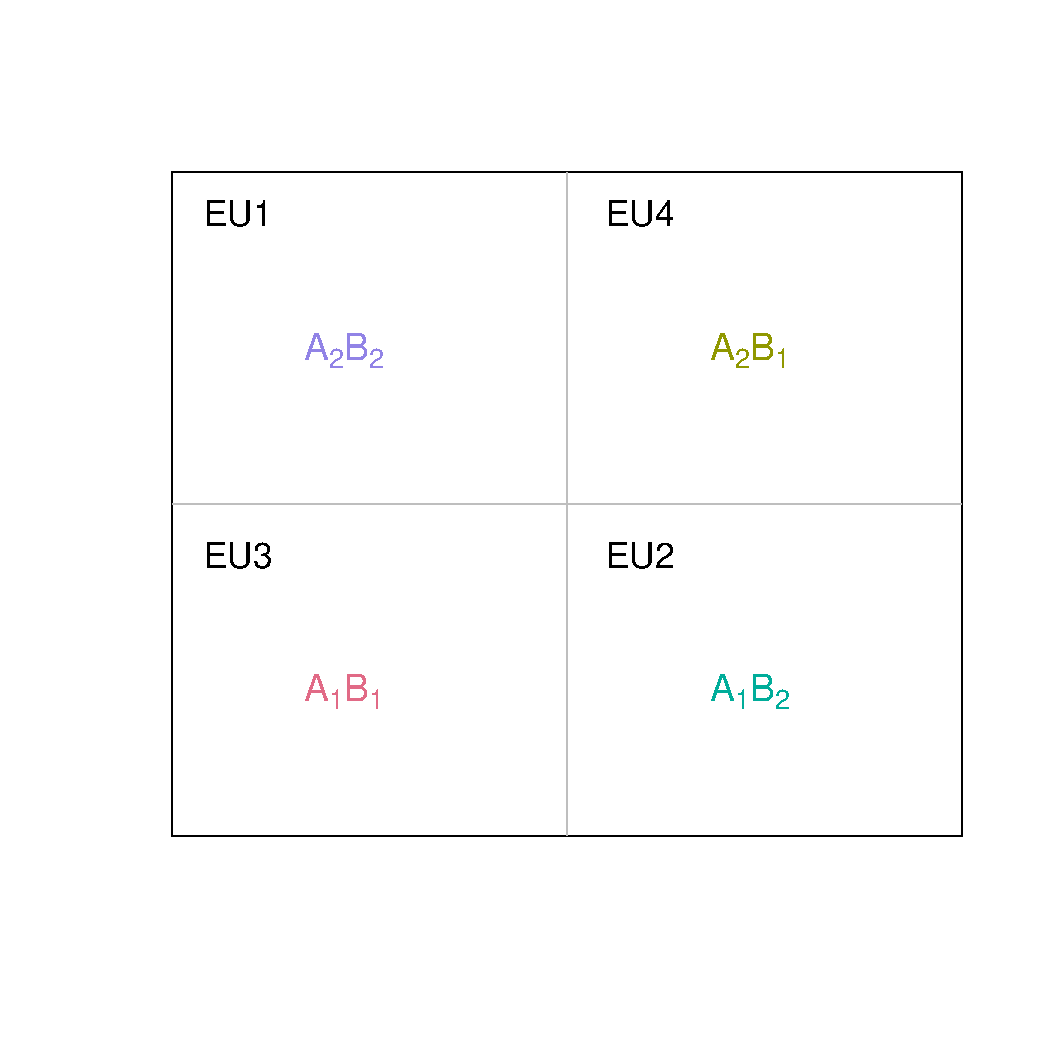
\includegraphics[width=.5\linewidth]{figure/minimal-unnamed-chunk-21-1} 

}


\end{knitrout}
\vspace{-.75in}
\caption{A 2 $\times$ 2 factorial design, i.e., two factors, $A$ and $B$, each with two levels. Four experimental units (EUs) are randomly assigned to one of four factor level combinations.  Thus, the design shown has no replication.}
\label{fig:fd}
\end{figure}

It should be emphasized that unbalanced multifactor designs should not be analyzed using the function \texttt{anova}.  This is because \texttt{anova} uses type I (sequential)sums of squares.  This will cause results to differ based on the order that factors are specified in the general linear model, i.e.,  \texttt{lm}.  With unbalanced multifactor designs one should the total sum of squares using a type II or type III sums of squares approach see \citep{aho2014}.  Type II sums of squares is the default method of \texttt{car::Anova} although Type III sums of squares can also be specified.
\par\noindent\rule{.9\textwidth}{0.4pt}
%%%%%%%%%%%%%%%%%%%%%%%%%%%%%%%%%%%%%%%%%%%%%%%%%%%%%%%%%%%%%%%%%%%%%%%%%%%%%%%%%%%%%%%%%%%%%%%%%%%%%%%%%%%%%%%%

\subsection{Two Way Factorial -- Two Fixed Factors}

\textbf{Model:} \[Y_{ijk} = \mu + \alpha_i + \beta_j + (\alpha\beta)_{ij} + \varepsilon_{ijk} \hspace{0.2in} \left\{
                \begin{array}{ll}
                  i = 1,2,\dots,a\\
                  j = 1,2,\dots,b\\
                  k = 1,2,\dots,n
                \end{array}
              \right.\]


\noindent where $Y_{ijk}$ is the \textit{k}th response for the \textit{i}th factor level from factor \textit{A} and the \textit{j}th factor level from factor \textit{B}, $\mu$ is the true grand mean, $\alpha_i$ is the \textit{i}th factor level effect, $\beta_j$ = is the \textit{j}th factor level effect, and $\varepsilon_{ijk}$ is the \textit{k}th error in the \textit{i}th factor level from \textit{A} and the \textit{j}th factor level from \textit{B}. \\
\vspace{0.05in}

\noindent \textbf{H$_0$:}
\begin{itemize}
\item $A$: $\mu_1 = \mu_2 = \dots = \mu_a$.
\item $B$: $\mu_1 = \mu_2 = \dots = \mu_b$.
\item \textit{A:B}: all $(\alpha\beta)_{ij} = 0$.
\end{itemize}
\vspace{0.1in}

\noindent \textbf{Assumptions:} $\varepsilon_{ijk} \sim N(0, \sigma^2)$.
\vspace{0.1in}

\noindent \textbf{Robust Alternatives:}
\begin{small}
\begin{itemize}
\item Brunner-Dette-Munk test \citep{brunner1997}, robust to outliers, non-normal errors and heteroscedasticity, \textbf{R:} \texttt{asbio::BDM.test}\vspace{-.1in}
\item Permutation tests \citep[see][]{manly2006}, \textbf{R:} \texttt{asbio::MC.test}
\end{itemize}
\end{small}
\vspace{0.1in}

\begin{tcolorbox}[colback=yellow!50!red!25!white,colbacktitle=yellow!50!red,colframe=black!75!white,title=\textbf{R:} Two Way Factorial -- Two Fixed Factors]
\textbf{Framework:}\\
\vspace{-.2in}
\begin{knitrout}
\definecolor{shadecolor}{rgb}{0.969, 0.969, 0.969}\color{fgcolor}\begin{kframe}
\begin{alltt}
\hlkwd{anova}\hldef{(}\hlkwd{lm}\hldef{(Y} \hlopt{~} \hldef{A} \hlopt{*} \hldef{B))}
\end{alltt}
\end{kframe}
\end{knitrout}
\vspace{-.1in}
or
\vspace{-.1in}
\begin{knitrout}
\definecolor{shadecolor}{rgb}{0.969, 0.969, 0.969}\color{fgcolor}\begin{kframe}
\begin{alltt}
\hlkwd{aov}\hldef{(Y} \hlopt{~} \hldef{A} \hlopt{*} \hldef{B)}
\end{alltt}
\end{kframe}
\end{knitrout}
where \texttt{Y} = response variable, and \texttt{A} and \texttt{B} are predictors, i.e., factors.
\vspace{0.1in}
\par\noindent\rule{.9\textwidth}{0.4pt}
\textbf{Example:} From \citep[][pg 65]{lawson}.  CO emissions were determined for combinations of three air/fuel ratios and three ethanol additions.
\vspace{-.1in}
\begin{knitrout}
\definecolor{shadecolor}{rgb}{0.969, 0.969, 0.969}\color{fgcolor}\begin{kframe}
\begin{alltt}
\hlkwd{library}\hldef{(daewr)}
\hlkwd{anova}\hldef{(}\hlkwd{lm}\hldef{(CO} \hlopt{~} \hldef{Eth} \hlopt{*} \hldef{Ratio,} \hlkwc{data} \hldef{= COdata))}
\end{alltt}
\end{kframe}
\end{knitrout}

\end{tcolorbox}
%%%%%%%%%%%%%%%%%%%%%%%%%%%%%%%%%%%%%%%%%%%%%%%%%%%%%%%%%%%%%%%%%%%%%%%%%%%%%%%%%%%%%%%%%%%%%%%%%%%%%%%%%%%%%
\par\noindent\rule{.9\textwidth}{0.4pt}

\subsection{Two Way Factorial -- One Fixed, One Random Factor}

\textbf{Model:} \[Y_{ijk} = \mu + \alpha_i + \beta_j + (\alpha\beta)_{ij} + \varepsilon_{ijk} \hspace{0.2in} \left\{
                \begin{array}{ll}
                  i = 1,2,\dots,a\\
                  j = 1,2,\dots,b\\
                  k = 1,2,\dots,n
                \end{array}
              \right.\]

 
\noindent where $Y_{ijk}$ is the \textit{k}th response for the \textit{i}th factor level from factor \textit{A} and the \textit{j}th factor level from random factor \textit{B}, $\mu$ is the true grand mean, $\alpha_i$ is the \textit{i}th factor level effect, $\beta_j$ = is the \textit{j}th random factor level effect, and $\varepsilon_{ijk}$ is the \textit{k}th error in the \textit{i}th factor level from \textit{A} and the \textit{j}th factor level from \textit{B}. \\
\vspace{0.05in}

\noindent \textbf{H$_0$:}
\begin{itemize}
\item $A$: $\mu_1 = \mu_2 = \dots = \mu_a$.
\item $B$: $\sigma^2_B = 0$.
\item \textit{A:B}: $\sigma^2_{AB}  = 0$.
\end{itemize}
\vspace{0.1in}

\noindent \textbf{Assumptions:} $\varepsilon_{ijk} \sim N(0, \sigma^2)$, \hspace{0.1in} $\beta_j \sim N(0 \sigma^2_B)$, \hspace{0.1in}  $(\alpha\beta)_{ij} \sim N(0, \sigma^2_{AB})$, \hspace{0.1in} $\beta_j \perp (\alpha\beta)_{ij}$, \hspace{0.1in}   $\beta_j,(\alpha\beta)_{ij} \perp \varepsilon_{ijk}$.
\vspace{0.1in}

\begin{tcolorbox}[colback=yellow!50!red!25!white,colbacktitle=yellow!50!red,colframe=black!75!white,title=\textbf{R:} Two Way Factorial -- One Fixed and One Random Factor]
\textbf{Framework:}\\
\vspace{-.2in}
\begin{knitrout}
\definecolor{shadecolor}{rgb}{0.969, 0.969, 0.969}\color{fgcolor}\begin{kframe}
\begin{alltt}
\hlkwd{library}\hldef{(nlme);} \hlkwd{library}\hldef{(car)}
\hlkwd{Anova}\hldef{(}\hlkwd{lme}\hldef{(Y} \hlopt{~} \hldef{A,} \hlkwc{random} \hldef{=} \hlnum{1}\hlopt{|}\hldef{B}\hlopt{/}\hldef{A))}
\end{alltt}
\end{kframe}
\end{knitrout}
\vspace{-.1in}
or
\vspace{-.1in}
\begin{knitrout}
\definecolor{shadecolor}{rgb}{0.969, 0.969, 0.969}\color{fgcolor}\begin{kframe}
\begin{alltt}
\hlkwd{library}\hldef{(lme4);} \hlkwd{library}\hldef{(lmerTest)}
\hldef{model} \hlkwb{<-} \hlkwd{lmer}\hldef{(Y} \hlopt{~} \hldef{A} \hlopt{+} \hldef{(}\hlnum{1}\hlopt{|}\hldef{B)} \hlopt{+} \hldef{(}\hlnum{1}\hlopt{|}\hldef{A}\hlopt{:}\hldef{B))}
\hlkwd{anova}\hldef{(model)} \hlcom{# fixed effects}
\hlkwd{ranova}\hldef{(model)} \hlcom{# random effects}
\end{alltt}
\end{kframe}
\end{knitrout}
\texttt{Y} = response variable, \texttt{A} is a fixed factor and \texttt{B} is a random factor.
\vspace{0.1in}
\par\noindent\rule{.9\textwidth}{0.4pt}
\textbf{Example:} From \citep[][pg 465]{aho2014}.   \citet{fisher1925} compared potato yield (per plant) for twelve potato varieties and three fertilizer treatments.
\vspace{-.1in}
\begin{knitrout}
\definecolor{shadecolor}{rgb}{0.969, 0.969, 0.969}\color{fgcolor}\begin{kframe}
\begin{alltt}
\hlkwd{library}\hldef{(asbio);} \hlkwd{data}\hldef{(potato)}
\hlkwd{library}\hldef{(lme4);} \hlkwd{library}\hldef{(lmerTest)}

\hlcom{# Anova(lme(Yield ~ Fert, random = ~ 1 | Variety/Fert,}
\hlcom{#           data = potato))}
\hlcom{# Take care with nesting specification with lme.  Fixed effect last.}

\hldef{model} \hlkwb{<-} \hlkwd{lmer}\hldef{(Yield} \hlopt{~} \hldef{Fert} \hlopt{+} \hldef{(}\hlnum{1}\hlopt{|}\hldef{Variety)} \hlopt{+} \hldef{(}\hlnum{1}\hlopt{|}\hldef{Variety}\hlopt{:}\hldef{Fert),}
           \hlkwc{data} \hldef{= potato)}
\hlkwd{anova}\hldef{(model)} \hlcom{# fixed effects}
\hlkwd{ranova}\hldef{(model)} \hlcom{# random effects}
\end{alltt}
\end{kframe}
\end{knitrout}
\end{tcolorbox}
%%%%%%%%%%%%%%%%
\par\noindent\rule{.9\textwidth}{0.4pt}

\subsection{Two Way Factorial -- Two Random Factors}

\textbf{Model:} \[Y_{ijk} = \mu + \alpha_i + \beta_j + (\alpha\beta)_{ij} + \varepsilon_{ijk} \hspace{0.2in} \left\{
                \begin{array}{ll}
                  i = 1,2,\dots,a\\
                  j = 1,2,\dots,b\\
                  k = 1,2,\dots,n
                \end{array}
              \right.\]


\noindent where $Y_{ijk}$ is the \textit{k}th response for the \textit{i}th factor level from random factor \textit{A} and the \textit{j}th factor level from random factor \textit{B}, $\mu$ is the true grand mean, $\alpha_i$ is the \textit{i}th random factor level effect, $\beta_j$ = is the \textit{j}th random factor level effect, and $\varepsilon_{ijk}$ is the \textit{k}th error in the \textit{i}th factor level from \textit{A} and the \textit{j}th factor level from \textit{B}. \\
\vspace{0.05in}

\noindent \textbf{H$_0$:}
\begin{itemize}
\item $A$: $\sigma^2_A = 0$.
\item $B$: $\sigma^2_B = 0$.
\item \textit{A:B}: $\sigma^2_{AB}  = 0$.
\end{itemize}
\vspace{0.1in}

\noindent \textbf{Assumptions:} $\varepsilon_{ijk} \sim N(0, \sigma^2)$, \hspace{0.1in} $\alpha_i \sim N(0, \sigma^2_A)$,\hspace{0.1in} $\beta_j \sim N(0, \sigma^2_B)$, \hspace{0.1in}  $(\alpha\beta)_{ij} \sim N(0, \sigma^2_{AB})$, \hspace{0.1in} $\alpha_i \perp \beta_j, (\alpha\beta)_{ij}$,\hspace{0.1in} $\beta_j \perp \alpha_i, (\alpha\beta)_{ij}$, \hspace{0.1in}   $\alpha_i, \beta_j,(\alpha\beta)_{ij} \perp \varepsilon_{ijk}$
\vspace{0.1in}

\begin{tcolorbox}[colback=yellow!50!red!25!white,colbacktitle=yellow!50!red,colframe=black!75!white,title=\textbf{R:} Two Random Factors]
\textbf{Framework:}\\

Note: \texttt{lme()} does not support crossed designs for random factors.

\vspace{-.1in}
\begin{knitrout}
\definecolor{shadecolor}{rgb}{0.969, 0.969, 0.969}\color{fgcolor}\begin{kframe}
\begin{alltt}
\hlkwd{library}\hldef{(lme4);} \hlkwd{library}\hldef{(lmerTest)}
\hldef{model} \hlkwb{<-} \hlkwd{lmer}\hldef{(score} \hlopt{~} \hlnum{1} \hlopt{+} \hldef{(}\hlnum{1}\hlopt{|}\hldef{A)} \hlopt{+} \hldef{(}\hlnum{1}\hlopt{|}\hldef{B)} \hlopt{+} \hldef{(}\hlnum{1}\hlopt{|}\hldef{A}\hlopt{:}\hldef{B))}
\hlkwd{anova}\hldef{(model)}
\hlkwd{ranova}\hldef{(model)}
\end{alltt}
\end{kframe}
\end{knitrout}
\texttt{Y} = response variable, and \texttt{A} and \texttt{B} are random factors.
\vspace{0.1in}
% \par\noindent\rule{.9\textwidth}{0.4pt}
\textbf{Example:}

\end{tcolorbox}
\par\noindent\rule{.9\textwidth}{0.4pt}


\subsection{Three Way Factorial (CRFD) -- Three Fixed Factors}

\textbf{Model:} \[Y_{ijkl} = \mu + \alpha_i + \beta_j + \gamma_k + (\alpha\beta)_{ij} + (\alpha\gamma)_{ik} + (\beta\gamma)_{jk} +  (\alpha\beta\gamma)_{ijk} + \varepsilon_{ijkl} \hspace{0.2in} \left\{
                \begin{array}{ll}
                  i = 1,2,\dots,a\\
                  j = 1,2,\dots,b\\
                  k = 1,2,\dots,c \\
                  l = 1,2,\dots,n \\
                \end{array}
              \right.\]


\noindent where $Y_{ijkl}$ is the \textit{l}th response for the \textit{i}th factor level from factor \textit{A}, the \textit{j}th factor level from factor \textit{B}, and the \textit{k}th factor level from factor \textit{C}, $\mu$ is the true grand mean, $\alpha_i$ is the \textit{i}th factor level effect, $\beta_j$ = is the \textit{j}th factor level effect, $\gamma_k$ = is the \textit{k}th factor level effect, and $\varepsilon_{ijk}$ is the \textit{l}th error in the \textit{i}th factor level from \textit{A}, the \textit{j}th factor level from \textit{B}, and the \textit{k}th factor level from \textit{C}. \\
\vspace{0.05in}

\noindent \textbf{H$_0$:}
\begin{itemize}
\item $A$: $\mu_1 = \mu_2 = \dots = \mu_a$.
\item $B$: $\mu_1 = \mu_2 = \dots = \mu_b$.
\item $C$: $\mu_1 = \mu_2 = \dots = \mu_c$.
\item \textit{A:B}: all $(\alpha\beta)_{ij} = 0$.
\item \textit{B:C}: all $(\beta\gamma)_{jk} = 0$.
\item \textit{A:C}: all $(\alpha\gamma)_{ik} = 0$.
\item \textit{A:B:C}: all $(\alpha\beta\gamma)_{ijk} = 0$.
\end{itemize}
\vspace{0.1in}

\noindent \textbf{Assumptions:} $\varepsilon_{ijkl} \sim N(0, \sigma^2)$.
\vspace{0.1in}

\begin{tcolorbox}[colback=yellow!50!red!25!white,colbacktitle=yellow!50!red,colframe=black!75!white,title=\textbf{R:} Three Fixed Factors]
\textbf{Framework:}\\
\vspace{-.2in}
\begin{knitrout}
\definecolor{shadecolor}{rgb}{0.969, 0.969, 0.969}\color{fgcolor}\begin{kframe}
\begin{alltt}
\hlkwd{anova}\hldef{(}\hlkwd{lm}\hldef{(Y} \hlopt{~} \hldef{A} \hlopt{*} \hldef{B} \hlopt{*} \hldef{C))}
\end{alltt}
\end{kframe}
\end{knitrout}
\vspace{-.1in}
or
\vspace{-.1in}
\begin{knitrout}
\definecolor{shadecolor}{rgb}{0.969, 0.969, 0.969}\color{fgcolor}\begin{kframe}
\begin{alltt}
\hlkwd{aov}\hldef{(Y} \hlopt{~} \hldef{A} \hlopt{*} \hldef{B} \hlopt{*} \hldef{C)}
\end{alltt}
\end{kframe}
\end{knitrout}
\texttt{Y} = response variable, and \texttt{A}, \texttt{B} and \texttt{C} are predictors, i.e., factors.
\vspace{0.1in}
\par\noindent\rule{.9\textwidth}{0.4pt}

\textbf{Example:} From \citep[][pg 83]{lawson}. This is a rather specialized example with a binomial response variable requiring a generalized linear model with a binomial error distribution and a logit link function.
\vspace{-.1in}
\begin{knitrout}
\definecolor{shadecolor}{rgb}{0.969, 0.969, 0.969}\color{fgcolor}\begin{kframe}
\begin{alltt}
\hlkwd{library}\hldef{(daewr)}
\hlkwd{data}\hldef{(web)}
\hldef{model} \hlkwb{<-} \hlkwd{glm}\hldef{(}\hlkwd{cbind}\hldef{(signup, visitors} \hlopt{-} \hldef{signup)} \hlopt{~} \hldef{A} \hlopt{*} \hldef{B} \hlopt{*} \hldef{C,}
             \hlkwc{data} \hldef{= web,} \hlkwc{family} \hldef{= binomial)}
\hlcom{# Note that the response variable can be entered as a}
\hlcom{# matrix containing the number of successes and the number of failures}
\hlkwd{anova}\hldef{(model,} \hlkwc{test} \hldef{=} \hlsng{"Chisq"}\hldef{)} \hlcom{# Likelihood-ratio test}
\end{alltt}
\end{kframe}
\end{knitrout}

\end{tcolorbox}
\par\noindent\rule{.9\textwidth}{0.4pt}
\newpage

\section{Randomized Block Designs}
In a \textit{randomized block design} a researcher randomly assigns experimental units to treatments separately within units called blocks.  Blocks are generally established to control for a potentially confounding background variable.

\subsection{Randomized Complete Block Design (RCBD)}
If all treatments are assigned exactly once within each block this is known as a \textit{randomized complete block design} or RCBD (Fig. \ref{fig:rcbd}).
\vspace{-.4in}

\begin{figure}[H]
\begin{knitrout}
\definecolor{shadecolor}{rgb}{0.969, 0.969, 0.969}\color{fgcolor}

{\centering 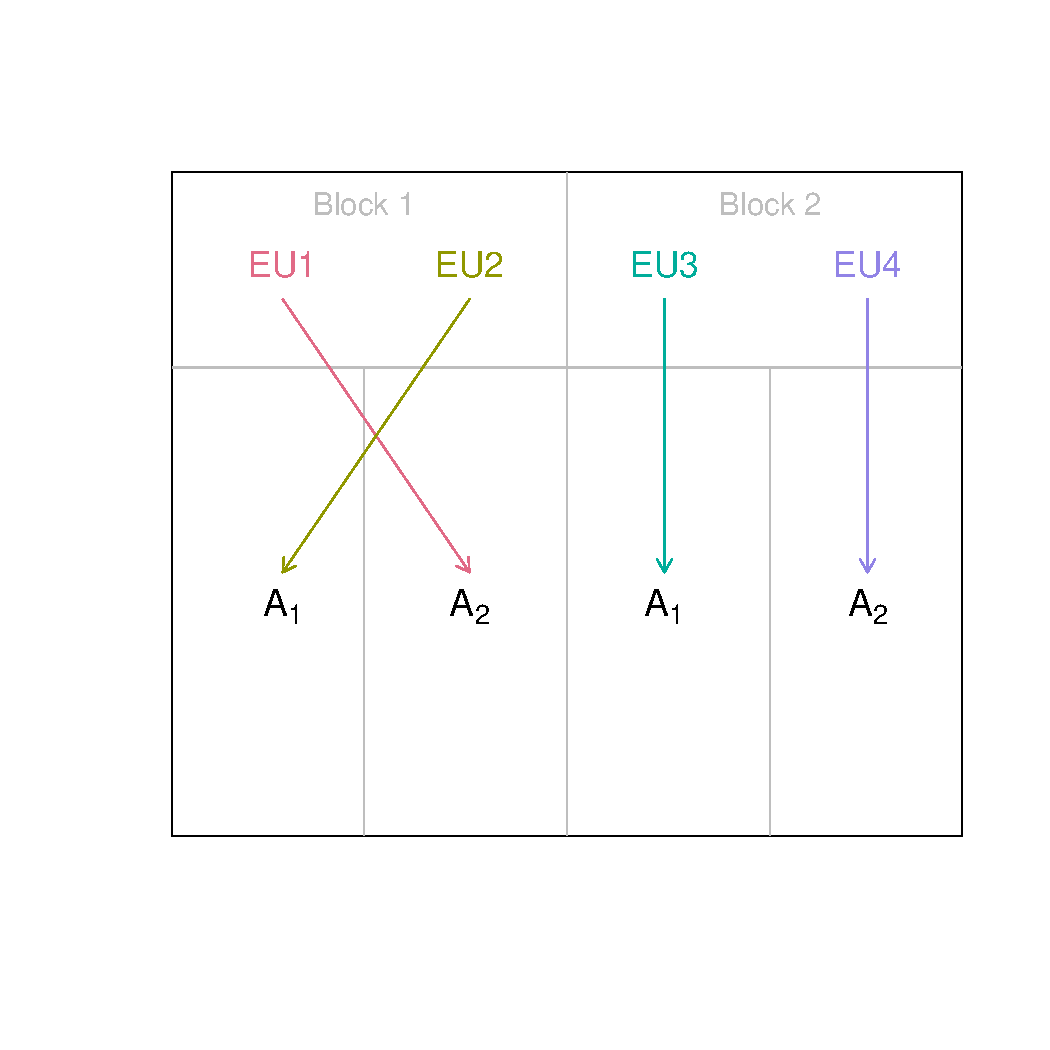
\includegraphics[width=.5\linewidth]{figure/minimal-unnamed-chunk-32-1} 

}


\end{knitrout}
\vspace{-.75in}
\caption{An RCBD with a factor of primary interest $A$, with two levels, and a blocking factor, $B$.  Two EUs within each of two blocks are randomly assigned to levels in $A$.}
\label{fig:rcbd}
\end{figure}

\noindent \textbf{Model:} \[Y_{ij} = \mu + \alpha_i + \beta_j + \varepsilon_{ij}  \hspace{0.2in} \left\{
                \begin{array}{ll}
                  i = 1,2,\dots,a\\
                  j = 1,2,\dots,b\\
              \end{array}
              \right.\]

\noindent where $Y_{ij}$ is the response for the \textit{i}th factor level in the $j$th block, $\mu$ is the true grand mean, $\alpha_i$ is the \textit{i}th factor level effect, $\beta_j$ is the $j$th block effect, and $\varepsilon_{ij}$ is the \textit{j}th block error in the \textit{i}th factor level. \\
\vspace{0.05in}

\noindent \textbf{H$_0$:}
\begin{itemize}
\item $A$: $\mu_1 = \mu_2 = \dots = \mu_a$.
\item $B$: $\mu_1 = \mu_2 = \dots = \mu_b$.
\end{itemize}
\vspace{0.1in}

\noindent \textbf{Assumptions:} $\varepsilon_{ij} \sim N(0, \sigma^2)$; all $(\alpha\beta)_{ij} = 0$
\vspace{0.1in}

\noindent \textbf{Robust Alternatives:}
\begin{small}
\begin{itemize}
\item Freidman test \citep{kruskal1952}, robust to non-normal errors, \textbf{R:} \texttt{freidman.test}\vspace{-.1in}
\item Agresti-Pendergrast test \citep{agresti1986}, more powerful than the Freidman test for most applications, \textbf{R:} \texttt{asbio::AP.test}
\end{itemize}
\end{small}
\vspace{0.1in}

\begin{tcolorbox}[colback=yellow!50!red!25!white,colbacktitle=yellow!50!red,colframe=black!75!white,title=\textbf{R:} RCBD]
\textbf{Framework:}\\
\vspace{-.2in}
\begin{knitrout}
\definecolor{shadecolor}{rgb}{0.969, 0.969, 0.969}\color{fgcolor}\begin{kframe}
\begin{alltt}
\hlkwd{anova}\hldef{(}\hlkwd{lm}\hldef{(Y} \hlopt{~} \hldef{A} \hlopt{+} \hldef{B))}
\end{alltt}
\end{kframe}
\end{knitrout}
\vspace{-.1in}
or
\vspace{-.1in}
\begin{knitrout}
\definecolor{shadecolor}{rgb}{0.969, 0.969, 0.969}\color{fgcolor}\begin{kframe}
\begin{alltt}
\hlkwd{aov}\hldef{(Y} \hlopt{~} \hldef{A} \hlopt{+} \hldef{B)}
\end{alltt}
\end{kframe}
\end{knitrout}
where \texttt{Y} = response variable, \texttt{A} = predictor, i.e., a factor, \texttt{B} = blocking variable.
\vspace{0.1in}
\par\noindent\rule{.9\textwidth}{0.4pt}

\textbf{Example:} From \citep[][Ex. 2.3.1]{hoshmand}
\vspace{-.1in}
\begin{knitrout}
\definecolor{shadecolor}{rgb}{0.969, 0.969, 0.969}\color{fgcolor}\begin{kframe}
\begin{alltt}
insects = \hlkwd{c}(8, 10, 18, 32, 12, 16, 26, 46, 16, 20, 26, 42, 10, 22, 20,
            40)
trap <- \hlkwd{as.factor}(\hlkwd{rep}(1:4, 4)) period <- \hlkwd{as.factor}(\hlkwd{rep}(1:4, each = 4))
\hlkwd{data.frame}(insects = insects, trap = trap, period = period)
\hlkwd{anova}(\hlkwd{lm}(insects ~ period + trap))
\end{alltt}
\end{kframe}
\end{knitrout}
\end{tcolorbox}

\par\noindent\rule{.9\textwidth}{0.4pt}

\subsection{RCBD with Random Blocks}

\textbf{Model:} \[Y_{ij} = \mu + \alpha_i + \beta_j + \varepsilon_{ij}\hspace{0.2in} \left\{
                \begin{array}{ll}
                  i = 1,2,\dots,a\\
                  j = 1,2,\dots,b\\
                  \end{array}
              \right.\]

where $Y_{ij}$ is the response for the \textit{i}th factor level in the $j$th random block, $\mu$ is the true grand mean, $\alpha_i$ is the \textit{i}th factor level effect, $\beta_j$ is the $j$th random block effect, and $\varepsilon_{ij}$ is the \textit{j}th error in the \textit{i}th factor level. \\
\vspace{0.05in}

\noindent \textbf{H$_0$:}
\begin{itemize}
\item $A$: $\mu_1 = \mu_2 = \dots = \mu_a$.
\item $B$: $\sigma^2_B = 0$.
\end{itemize}
\vspace{0.1in}

\noindent \textbf{Assumptions:} $\varepsilon_{ij} \sim N(0, \sigma^2)$, \hspace{0.1in} $\beta_j \sim N(0, \sigma^2_B)$, \hspace{0.1in} $\beta_j \perp \varepsilon_{ij}$, \hspace{0.1in} all $(\alpha\beta)_{ij} = 0$.
\vspace{0.1in}

\begin{tcolorbox}[colback=yellow!50!red!25!white,colbacktitle=yellow!50!red,colframe=black!75!white,title=\textbf{R:} RCBD With Random Blocks]
\textbf{Framework:}\\
\vspace{-.2in}
\begin{knitrout}
\definecolor{shadecolor}{rgb}{0.969, 0.969, 0.969}\color{fgcolor}\begin{kframe}
\begin{alltt}
\hlkwd{library}\hldef{(lme4);} \hlkwd{library}\hldef{(lmerTest)}
\hldef{model} \hlkwb{<-} \hlkwd{lmer}\hldef{(Y} \hlopt{~} \hldef{A} \hlopt{+} \hldef{(}\hlnum{1}\hlopt{|}\hldef{B))}
\hlkwd{anova}\hldef{(model)} \hlcom{# fixed}
\hlkwd{ranova}\hldef{(model)} \hlcom{# random}
\end{alltt}
\end{kframe}
\end{knitrout}
\texttt{Y} = response variable, \texttt{A} = predictor, i.e., a factor, \texttt{B} = random blocking variable.
\vspace{0.1in}
\par\noindent\rule{.9\textwidth}{0.4pt}

\textbf{Example:} From \citep[][]{pinheiro2009} Nine testers had to sit in four different ergonomic stools. The effort required to raise the stool was measured once.
\vspace{-.1in}
\begin{knitrout}
\definecolor{shadecolor}{rgb}{0.969, 0.969, 0.969}\color{fgcolor}\begin{kframe}
\begin{alltt}
\hlkwd{library}\hldef{(lme4);} \hlkwd{library}\hldef{(lmerTest);} \hlkwd{library}\hldef{(nlme)} \hlcom{#nlme contains ergostool}
\hldef{model} \hlkwb{<-} \hlkwd{lmer}\hldef{(effort} \hlopt{~} \hldef{Type} \hlopt{+} \hldef{(}\hlnum{1} \hlopt{|} \hldef{Subject),}
             \hlkwc{data} \hldef{= ergoStool)}
\hlkwd{anova}\hldef{(model)} \hlcom{# fixed}
\hlkwd{ranova}\hldef{(model)} \hlcom{# random}
\end{alltt}
\end{kframe}
\end{knitrout}
\end{tcolorbox}

\par\noindent\rule{.9\textwidth}{0.4pt}


\subsection{Generalized Complete Block Design (GCB) - i.e. replicated RCBD}

\textbf{Model:} \[Y_{ijk} = \mu + \alpha_i + \beta_j +  (\alpha\beta)_{ij} + \varepsilon_{ijk}\hspace{0.2in} \left\{
                \begin{array}{ll}
                  i = 1,2,\dots,a\\
                  j = 1,2,\dots,b\\
                  k = 1,2,\dots, n\\
                                 \end{array}
              \right.\]

\noindent where $Y_{ijk}$ is the \textit{k}th response for the \textit{i}th factor level in the $j$th block, $\mu$ is the true grand mean, $\alpha_i$ is the \textit{i}th factor level effect, $\beta_j$ is the $j$th block effect, $(\alpha\beta)_{ij}$ is the interaction effect of the factor and block, and $\varepsilon_{ij}$ is the \textit{j}th error in the \textit{i}th factor level. \\
\vspace{0.05in}

\noindent \textbf{H$_0$:}
\begin{itemize}
\item $A$: $\mu_1 = \mu_2 = \dots = \mu_A$.
\item $B$: $\mu_1 = \mu_2 = \dots = \mu_B$.
\item \textit{A:B}: all $(\alpha\beta)_{ij} = 0$.
\end{itemize}
\vspace{0.1in}

\noindent \textbf{Assumptions:} $\varepsilon_{ijk} \sim N(0, \sigma^2)$
\vspace{0.1in}

\noindent \textbf{Robust Alternatives:}
\begin{small}
\begin{itemize}
\item Mack-Skillings test \citep{mack1980}, robust to violation of normal errors, \textbf{R:} \texttt{asbio::MS.test}
\end{itemize}
\end{small}
\vspace{0.1in}

\begin{tcolorbox}[colback=yellow!50!red!25!white,colbacktitle=yellow!50!red,colframe=black!75!white,title=\textbf{R:} GCB]
\textbf{Framework:}\\
\vspace{-.2in}
\begin{knitrout}
\definecolor{shadecolor}{rgb}{0.969, 0.969, 0.969}\color{fgcolor}\begin{kframe}
\begin{alltt}
\hlcom{# At least initially one should use:}
\hlkwd{aov}\hldef{(Y} \hlopt{~} \hldef{A} \hlopt{+} \hlkwd{Error}\hldef{(B}\hlopt{/}\hldef{A))}
\hlcom{# Lack of an interaction would prompt use of}
\hlkwd{aov}\hldef{(Y} \hlopt{~} \hldef{A} \hlopt{*} \hldef{B)}
\end{alltt}
\end{kframe}
\end{knitrout}

where \texttt{Y} = response variable, \texttt{A} = predictor, i.e., a factor, \texttt{B} = blocking variable.
\vspace{0.1in}
\par\noindent\rule{.9\textwidth}{0.4pt}

\textbf{Example:} From \citep[][pgs 125-128]{lawson}
\vspace{-.1in}
\begin{knitrout}
\definecolor{shadecolor}{rgb}{0.969, 0.969, 0.969}\color{fgcolor}\begin{kframe}
\begin{alltt}
\hlkwd{library}\hldef{(daewr)}
\hlkwd{smmary}\hldef{(}\hlkwd{aov}\hldef{(cdistance} \hlopt{~} \hldef{teeht} \hlopt{+} \hlkwd{Error}\hldef{(id}\hlopt{/}\hldef{teeht),} \hlkwc{data} \hldef{= rcb))}
\end{alltt}
\end{kframe}
\end{knitrout}
\end{tcolorbox}
\par\noindent\rule{.9\textwidth}{0.4pt}


\subsection{Latin Square Design (LSD)}
\textit{Latin squares designs} are useful when there are two potential blocking variables. These can figuratively or literally be represented by rows and columns. All treatments are assigned to each row and to each column, and for each row and column treatment assignments differ. Of course this stipulation limits the number of ways one can allocate treatments.
\vspace{-.4in}
\begin{figure}[H]
\begin{knitrout}
\definecolor{shadecolor}{rgb}{0.969, 0.969, 0.969}\color{fgcolor}

{\centering 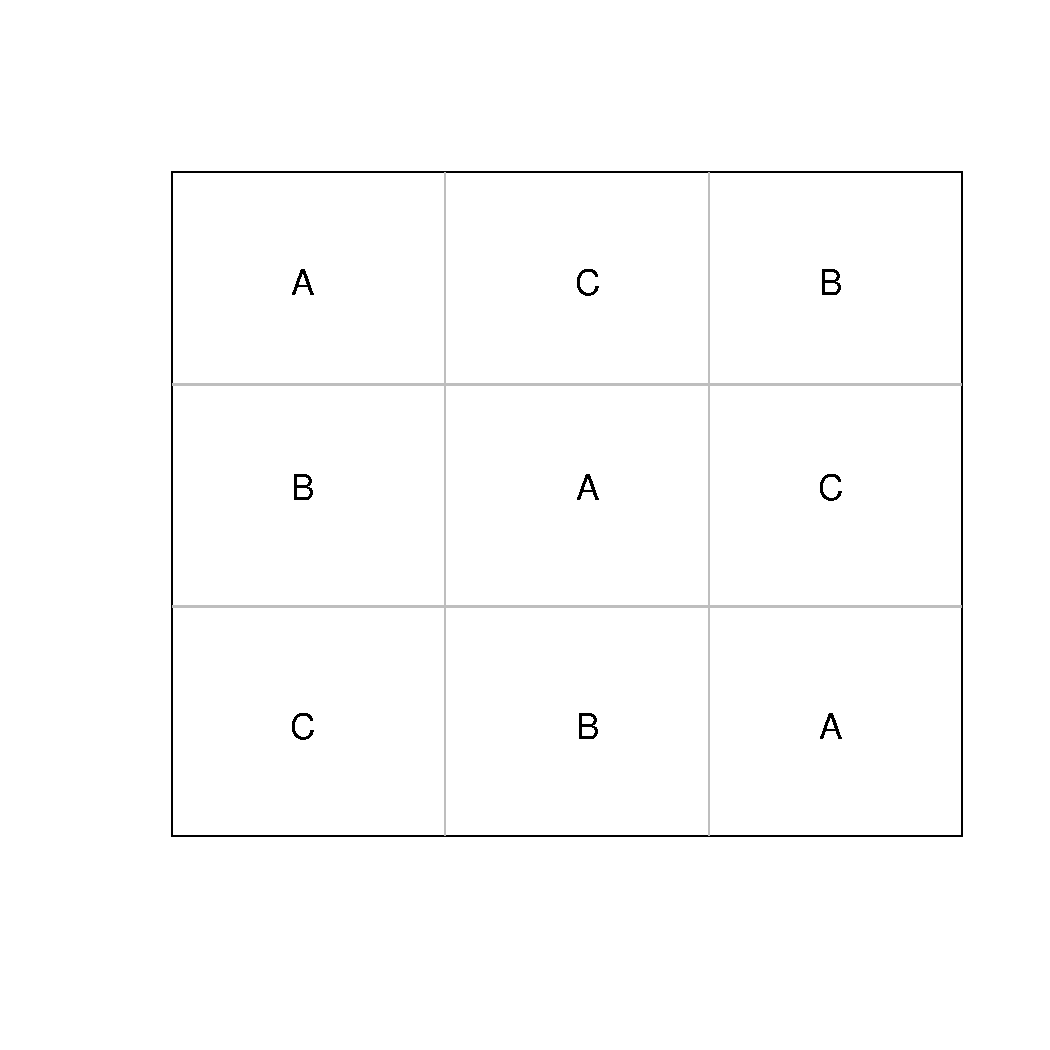
\includegraphics[width=.5\linewidth]{figure/minimal-unnamed-chunk-40-1} 

}


\end{knitrout}
\vspace{-.75in}
\caption{A three row and three column Latin squares design.  Three treatments (A,B,C) are randomly assigned so that each treatment occurs once in each row and once in each column.}
\label{fig:fd1}
\end{figure}

\noindent\textbf{Model:} \[Y_{ijk} = \mu + \alpha_i + \beta_j +  \gamma_k  + \varepsilon_{ijk} \hspace{0.2in} \left\{
                \begin{array}{ll}
                  i = 1,2,\dots,a\\
                  j = 1,2,\dots,b\\
                  k = 1,2,\dots,c \\
                                  \end{array}
              \right.\]

\noindent where $Y_{ijk}$ is the response for the \textit{i}th factor level in the $j$th row and the $k$th column, $\mu$ is the true grand mean, $\alpha_i$ is the \textit{i}th factor level effect, $\beta_j$ is the $j$th row blocking effect, $\gamma_k$ is the $k$th column blocking effect, and $\varepsilon_{ijk}$ is the \textit{k}th error in the \textit{i}th row and the \textit{k}th column. \\
\vspace{0.05in}

\noindent \textbf{H$_0$:}
\begin{itemize}
\item $A$: $\mu_1 = \mu_2 = \dots = \mu_A$.
\item $B$: $\mu_1 = \mu_2 = \dots = \mu_B$.
\item $C$: $\mu_1 = \mu_2 = \dots = \mu_C$.
\end{itemize}
\vspace{0.1in}

\noindent \textbf{Assumptions:} $\varepsilon_{ijk} \sim N(0, \sigma^2)$, \hspace{0.1in} $(\alpha\beta)_{ij} = 0$, \hspace{0.1in}
$(\alpha\gamma)_{ik} = 0$, \hspace{0.1in} $(\alpha\beta\gamma)_{ijk} = 0$
\vspace{0.1in}

\begin{tcolorbox}[colback=yellow!50!red!25!white,colbacktitle=yellow!50!red,colframe=black!75!white,title=\textbf{R:} LSD]
\textbf{Framework:}\\
\vspace{-.2in}
\begin{knitrout}
\definecolor{shadecolor}{rgb}{0.969, 0.969, 0.969}\color{fgcolor}\begin{kframe}
\begin{alltt}
\hlkwd{anova}\hldef{(}\hlkwd{lm}\hldef{(Y} \hlopt{~} \hldef{X} \hlopt{+} \hldef{R} \hlopt{+} \hldef{C))}
\end{alltt}
\end{kframe}
\end{knitrout}
\vspace{-.1in}
or
\vspace{-.1in}
\begin{knitrout}
\definecolor{shadecolor}{rgb}{0.969, 0.969, 0.969}\color{fgcolor}\begin{kframe}
\begin{alltt}
\hlkwd{aov}\hldef{(Y} \hlopt{~} \hldef{X} \hlopt{+} \hldef{R} \hlopt{+} \hldef{C)}
\end{alltt}
\end{kframe}
\end{knitrout}

\texttt{Y} = response variable, \texttt{X} = predictor, \texttt{R} = row blocking variable, \texttt{C} = column blocking variable.
\vspace{0.1in}
\par\noindent\rule{.9\textwidth}{0.4pt}

\textbf{Example:} \citep[][pg 72]{litt2002}.  Permanent press garments were subjected to a test for shrinkage.  In particular, four materials were placed in a heat chamber with four control settings over four runs with each material assigned to one of each of the four position in one execution of the experiment.
\vspace{-.1in}
\begin{knitrout}
\definecolor{shadecolor}{rgb}{0.969, 0.969, 0.969}\color{fgcolor}\begin{kframe}
\begin{alltt}
\hlkwd{library}\hldef{(asbio);} \hlkwd{data}\hldef{(garments)}
\hlkwd{anova}\hldef{(}\hlkwd{lm}\hldef{(shrink} \hlopt{~} \hldef{mat} \hlopt{+} \hldef{pos} \hlopt{+} \hldef{run,} \hlkwc{data} \hldef{= garments))}
\end{alltt}
\end{kframe}
\end{knitrout}
\end{tcolorbox}
\newpage
\section{Fractional Factorial Designs}
\textit{Fractional factorial designs} consist of a carefully chosen subset of the experimental runs of a full factorial design.  \textbf{Under construction}
\par\noindent\rule{.9\textwidth}{0.4pt}

\newpage
\section{Incomplete and Confounded Block Designs}
\subsection{Balanced Incomplete Block Design (BIBD)}
\vspace{-.4in}
\begin{figure}[H]
\begin{knitrout}
\definecolor{shadecolor}{rgb}{0.969, 0.969, 0.969}\color{fgcolor}

{\centering 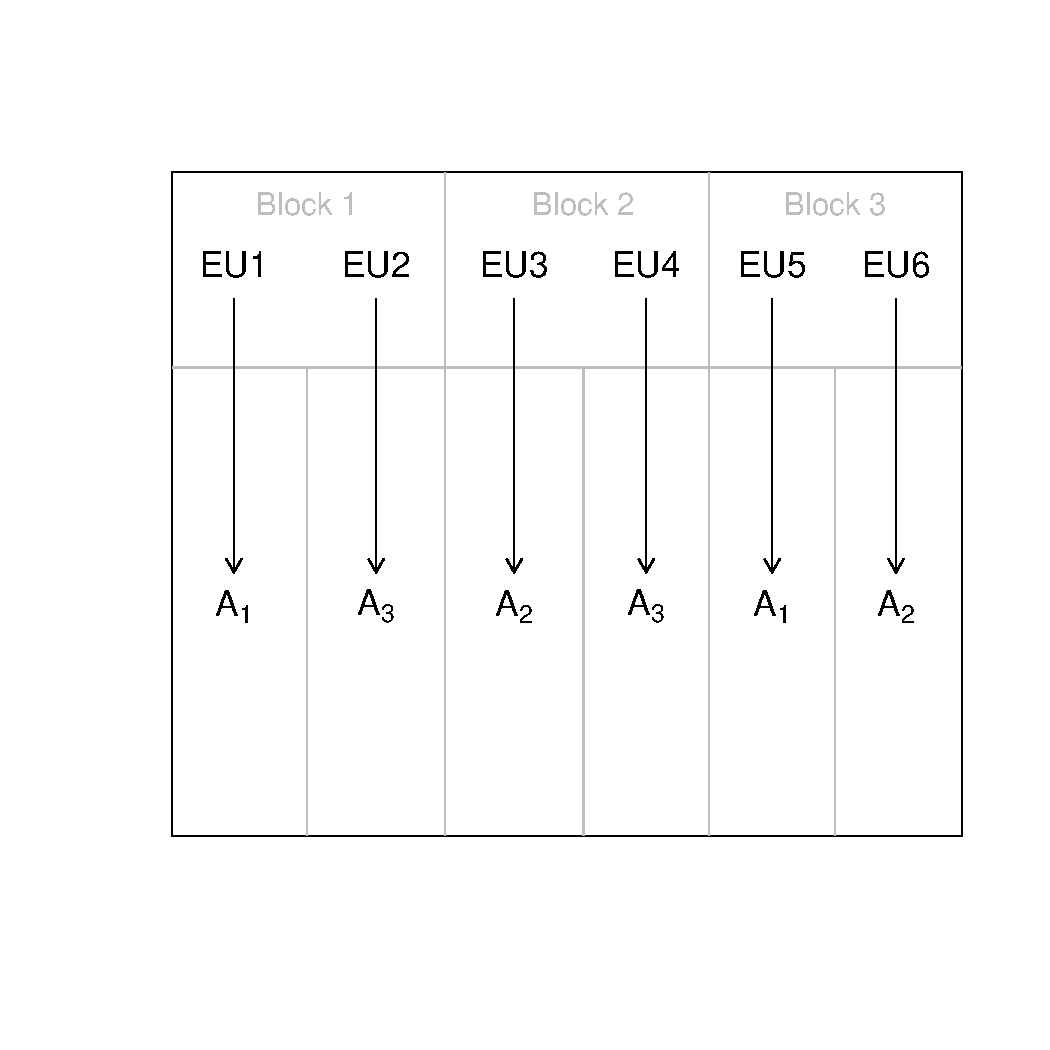
\includegraphics[width=.5\linewidth]{figure/minimal-unnamed-chunk-44-1} 

}


\end{knitrout}
\vspace{-.75in}
\caption{An BIBD with a factor of primary interest $A$, with three levels, and a blocking factor, $B$.  Two EUs within each of three blocks are randomly assigned to the three levels in $A$.  The three levels have equal replication, $n = 2$}
\label{fig:ribd}
\end{figure}

\noindent \textbf{Model:} \[Y_{ij} = \mu + \alpha_i + \beta_j + \varepsilon_{ij} \hspace{0.2in} \left\{
                \begin{array}{ll}
                  i = 1,2,\dots,a\\
                  j = 1,2,\dots,b\\
                  \end{array}
              \right.\]

\noindent where $Y_{ij}$ is the response for the \textit{i}th factor level in the $j$th block, $\mu$ is the true grand mean, $\alpha_i$ is the \textit{i}th factor level effect, $\beta_j$ is the $j$th block effect, and $\varepsilon_{ij}$ is the \textit{j}th block error in the \textit{i}th factor level. \\
\vspace{0.05in}

\noindent \textbf{H$_0$:}
\begin{itemize}
\item $A$: $\mu_1 = \mu_2 = \dots = \mu_a$.
\item $B$: $\mu_1 = \mu_2 = \dots = \mu_b$.
\end{itemize}
\vspace{0.1in}

\noindent \textbf{Assumptions:} $\varepsilon_{ij} \sim N(0, \sigma^2)$, all $(\alpha\beta)_{ij} = 0$
\vspace{0.1in}


\begin{tcolorbox}[colback=yellow!50!red!25!white,colbacktitle=yellow!50!red,colframe=black!75!white,title=\textbf{R:} BIBD]
\textbf{Framework:}\\
\vspace{-.2in}
\begin{knitrout}
\definecolor{shadecolor}{rgb}{0.969, 0.969, 0.969}\color{fgcolor}\begin{kframe}
\begin{alltt}
\hlkwd{library}\hldef{(car)}
\hlkwd{Anova}\hldef{(}\hlkwd{lm}\hldef{(Y} \hlopt{~} \hldef{A} \hlopt{*} \hldef{B),} \hlkwc{type} \hldef{=} \hlsng{"III"}\hldef{)}
\end{alltt}
\end{kframe}
\end{knitrout}
\texttt{Y} = response variable, \texttt{A} is a predictor i.e., factor, and \texttt{B} is an (incomplete) blocking factor.
\vspace{0.1in}
\par\noindent\rule{.9\textwidth}{0.4pt}


\textbf{Example:} From \citep[][pg 267]{lawson}.  A taste panel experiment was run in which twelve panelists (blocks) were randomly assigned to two of four recipes.
\vspace{-.1in}
\begin{knitrout}
\definecolor{shadecolor}{rgb}{0.969, 0.969, 0.969}\color{fgcolor}\begin{kframe}
\begin{alltt}
\hlkwd{library}\hldef{(daewr);} \hlkwd{library}\hldef{(car)}
\hlkwd{data}\hldef{(taste)}
\hlkwd{Anova}\hldef{(}\hlkwd{lm}\hldef{(score} \hlopt{~} \hldef{recipe} \hlopt{+} \hldef{panelist,} \hlkwc{data} \hldef{= taste),} \hlkwc{type} \hldef{=} \hlsng{"III"}\hldef{)}
\end{alltt}
\end{kframe}
\end{knitrout}

\end{tcolorbox}
\par\noindent\rule{.9\textwidth}{0.4pt}
\subsection{Partialy Balanced Incomplete Block Design (PBIB)}
Balanced With Respect to Control (BTIB)
\par\noindent\rule{.9\textwidth}{0.4pt}
\subsection{Confounded $2^k$ and $2^{k-p}$ Design}
\par\noindent\rule{.9\textwidth}{0.4pt}
\subsection{Partially Confounded Blocked Factorial Design (PCBF)}
\par\noindent\rule{.9\textwidth}{0.4pt}
\newpage

\section{Nested Designs (NSE)}
In a \textit{nested sampling experiment} (NSE), factor levels from one factor will be contained entirely in one factor level from another factor. Consider a design with two factors $A$ and $B$. When every level of factor $A$ appears with every level of factor $B$, and \textit{vice versa}, then we have a fully crossed factorial design (see above). Conversely, when levels of $B$ only occur within a single level of $A$, then $B$ is nested in $A$.
\vspace{-.4in}
\begin{figure}[H]
\begin{knitrout}
\definecolor{shadecolor}{rgb}{0.969, 0.969, 0.969}\color{fgcolor}

{\centering 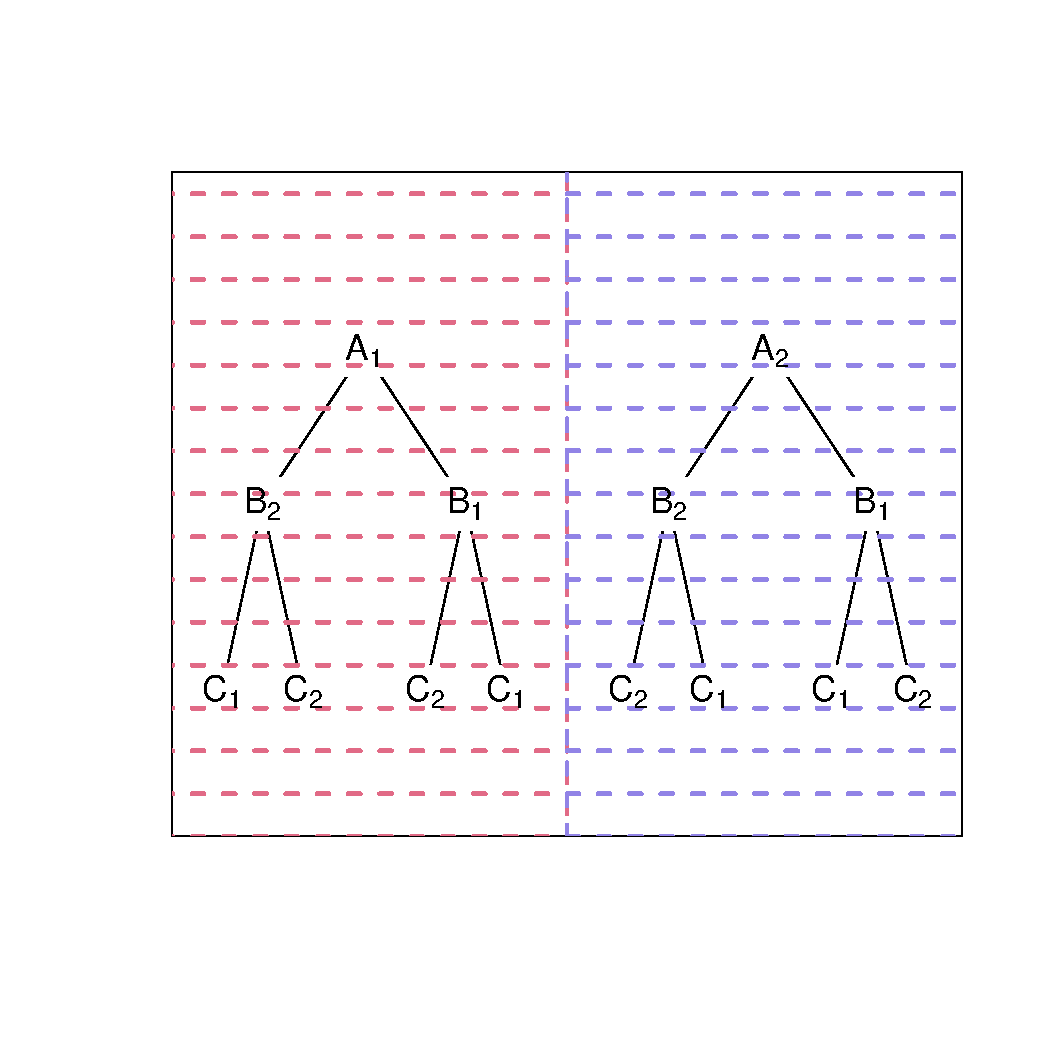
\includegraphics[width=.5\linewidth]{figure/minimal-unnamed-chunk-47-1} 

}


\end{knitrout}
\vspace{-.75in}
\caption{A three stage nested design with two independent observations, each with two levels of nested subsampling.}
\label{fig:nd}
\end{figure}

\subsection{Two Stage Nested Design -- One Random Nested Factor}
\textbf{Model:} \[Y_{ijk} = \mu + \alpha_i + \beta_{j(i)} +(\alpha\beta)_{j(i)} + \varepsilon_{ijk} \hspace{0.2in} \left\{
                \begin{array}{ll}
                  i = 1,2,\dots,a\\
                  j = 1,2,\dots,b\\
                  k = 1,2,\dots,n\\
                  \end{array}
              \right.\]

\noindent where $Y_{ijk}$ is the \textit{k}th response for the $j$th level of $B$, nested in the \textit{i}th factor level of $A$, $\mu$ is the true grand mean, $\alpha_i$ is the \textit{i}th factor level effect, $\beta_{j(i)}$ is the $j$th factor level in $B$ in the $ith$ level in $A$, and $\varepsilon_{ijk}$ is the \textit{k}th error in the \textit{i}th factor level in $A$ and the $j$th level in $B$. \\
\vspace{0.05in}

\noindent \textbf{H$_0$:}
\begin{itemize}
\item $A$: $\mu_1 = \mu_2 = \dots = \mu_a$.
\item $B$: $\sigma^2_B = 0$.
\item \textit{A:B}: $\sigma^2_{AB} = 0$.
\end{itemize}
\vspace{0.1in}

\noindent \textbf{Assumptions:} $\varepsilon_{ijk} \sim N(0, \sigma^2)$, \hspace{0.1in} $\beta_{j(i)} \sim N(0, \sigma^2_B)$, \hspace{0.1in} $\beta_{j(i)} \perp \varepsilon_{ijk}$.
\vspace{0.1in}

\begin{tcolorbox}[colback=yellow!50!red!25!white,colbacktitle=yellow!50!red,colframe=black!75!white,title=\textbf{R:} NSE - One Random Nested Factor]
\textbf{Framework:}\\
\vspace{-.2in}
\begin{knitrout}
\definecolor{shadecolor}{rgb}{0.969, 0.969, 0.969}\color{fgcolor}\begin{kframe}
\begin{alltt}
\hlkwd{library}\hldef{(lme4);} \hlkwd{library}\hldef{(car)}
\hldef{model} \hlkwb{<-} \hlkwd{lmer}\hldef{(Y} \hlopt{~} \hldef{A} \hlopt{+} \hldef{(}\hlnum{1}\hlopt{|}\hldef{B)} \hlopt{+} \hldef{(}\hlnum{1}\hlopt{|}\hldef{A}\hlopt{:}\hldef{B))}
\hlkwd{anova}\hldef{(model)}
\hlkwd{ranova}\hldef{(model)}
\end{alltt}
\end{kframe}
\end{knitrout}
\texttt{Y} = response variable, \texttt{A} is a fixed factor, \texttt{B} is a random factor nested in \texttt{A}.
\vspace{0.1in}
\par\noindent\rule{.9\textwidth}{0.4pt}

\textbf{Example:} From \citep[][pgs 156-159]{lawson}.  In a quality assurance analysis 10 parts were considered, each with three nested operators.  Two observations were obtained per operator.
\vspace{0.1in}\\

\vspace{-.1in}
\begin{knitrout}
\definecolor{shadecolor}{rgb}{0.969, 0.969, 0.969}\color{fgcolor}\begin{kframe}
\begin{alltt}
\hlkwd{library}\hldef{(daewr);} \hlkwd{data}\hldef{(gagerr)}
\hlkwd{library}\hldef{(lme4);} \hlkwd{library}\hldef{(car);} \hlkwd{library}\hldef{(lmerTest)}
\hldef{model} \hlkwb{<-} \hlkwd{lmer}\hldef{(y} \hlopt{~} \hldef{part} \hlopt{+} \hldef{(}\hlnum{1}\hlopt{|}\hldef{oper)} \hlopt{+} \hldef{(}\hlnum{1}\hlopt{|}\hldef{part}\hlopt{:}\hldef{oper),}
              \hlkwc{data} \hldef{= gagerr)}
\hlkwd{anova}\hldef{(model)} \hlcom{# fixed effects}
\hlkwd{ranova}\hldef{(model)} \hlcom{# random effects}
\end{alltt}
\end{kframe}
\end{knitrout}
\end{tcolorbox}
\par\noindent\rule{.9\textwidth}{0.4pt}



\subsection{Two Stage Nested Design -- Both Factors Random}
\textbf{Model:} \[Y_{ijk} = \mu + \alpha_i + \beta_{j(i)} +(\alpha\beta)_{j(i)}+ \varepsilon_{ijk} \hspace{0.2in} \left\{
                \begin{array}{ll}
                  i = 1,2,\dots,a\\
                  j = 1,2,\dots,b\\
                  k = 1,2,\dots,n\\
                  \end{array}
              \right.\]

\noindent where $Y_{ijk}$ is the \textit{k}th response for the $j$th level of $B$, nested in the \textit{i}th factor level of $A$, $\mu$ is the true grand mean, $\alpha_i$ is the \textit{i}th factor level effect, $\beta_{j(i)}$ is the $j$th factor level in $B$ in the $ith$ level in $A$, and $\varepsilon_{ijk}$ is the \textit{k}th error in the \textit{i}th factor level in $A$ and the $j$th level in $B$. \\
\vspace{0.05in}

\noindent \textbf{H$_0$:}
\begin{itemize}
\item $A$: $\sigma^2_A = 0$.
\item $B$: $\sigma^2_B = 0$.
\item \textit{A:B}: $\sigma^2_{AB} = 0$.
\end{itemize}
\vspace{0.1in}
\noindent \textbf{Assumptions:} $\varepsilon_{ijk} \sim N(0, \sigma^2)$, \hspace{0.1in} $\alpha_i \sim N(0, \sigma^2_A)$,\hspace{0.1in} $\beta_j \sim N(0, \sigma^2_B)$, \hspace{0.1in}  $(\alpha\beta)_{ij} \sim N(0, \sigma^2_{AB})$, \hspace{0.1in} $\alpha_i \perp \beta_j, (\alpha\beta)_{ij}$,\hspace{0.1in} $\beta_j \perp \alpha_i, (\alpha\beta)_{ij}$, \hspace{0.1in}   $\alpha_i, \beta_j,(\alpha\beta)_{ij} \perp \varepsilon_{ijk}$
\vspace{0.1in}

\begin{tcolorbox}[colback=yellow!50!red!25!white,colbacktitle=yellow!50!red,colframe=black!75!white,title=\textbf{R:} NSE - Both Factors Random]
\textbf{Framework:}\\
\vspace{-.2in}
\begin{knitrout}
\definecolor{shadecolor}{rgb}{0.969, 0.969, 0.969}\color{fgcolor}\begin{kframe}
\begin{alltt}
\hlkwd{library}\hldef{(lme4);} \hlkwd{library}\hldef{(lmerTest)}
\hldef{model} \hlkwb{<-} \hlkwd{lmer}\hldef{(Y} \hlopt{~} \hldef{(}\hlnum{1}\hlopt{|}\hldef{A)} \hlopt{+} \hldef{(}\hlnum{1}\hlopt{|}\hldef{B)} \hlopt{+} \hldef{(}\hlnum{1}\hlopt{|}\hldef{A}\hlopt{:}\hldef{B))}
\hlkwd{ranova}\hldef{(model)}
\end{alltt}
\end{kframe}
\end{knitrout}
\texttt{Y} = response variable, \texttt{A} is a fixed factor, \texttt{B} is a random factor nested in \texttt{A}.
\vspace{0.1in}
\par\noindent\rule{.9\textwidth}{0.4pt}

\textbf{Example:} \citet[][pgs 156-159]{lawson} treated both explanatory variables in the gage dataset as random.

\begin{knitrout}
\definecolor{shadecolor}{rgb}{0.969, 0.969, 0.969}\color{fgcolor}\begin{kframe}
\begin{alltt}
\hlkwd{library}\hldef{(daewr);} \hlkwd{data}\hldef{(gagerr)}
\hlkwd{library}\hldef{(lme4);} \hlkwd{library}\hldef{(lmerTest)}
\hldef{model} \hlkwb{<-} \hlkwd{lmer}\hldef{(y} \hlopt{~} \hldef{(}\hlnum{1}\hlopt{|}\hldef{part)} \hlopt{+} \hldef{(}\hlnum{1}\hlopt{|}\hldef{oper)} \hlopt{+} \hldef{(}\hlnum{1}\hlopt{|}\hldef{part}\hlopt{:}\hldef{oper),}
              \hlkwc{data} \hldef{= gagerr)}
\hlkwd{ranova}\hldef{(model)} \hlcom{# random effects}
\end{alltt}
\end{kframe}
\end{knitrout}
\end{tcolorbox}
\par\noindent\rule{.9\textwidth}{0.4pt}

\subsection{Three Stage Nested Design -- Two Random Nested Factors}
\textbf{Model:} \[Y_{ijkl} = \mu + \alpha_i + \beta_{j(i)} +\gamma_{k(ij)} + \varepsilon_{ijkl} \hspace{0.2in} \left\{
                \begin{array}{ll}
                  i = 1,2,\dots,a\\
                  j = 1,2,\dots,b\\
                  k = 1,2,\dots,c\\
                  l = 1,2,\dots,n\\
                  \end{array}
              \right.\]

\noindent where $Y_{ijkl}$ is the \textit{l}th response from the $k$th level in $C$, nested in the $j$th level of $B$, nested in the \textit{i}th level of $A$, $\mu$ is the true grand mean, $\alpha_i$ is the \textit{i}th factor level effect, $\beta_{j(i)}$ is the $j$th factor level in $B$ in the $i$th level in $A$, $\gamma_{k(ij)}$ is the $k$th factor level in $C$ in the $j$th level in $B$, and the $i$th level in $A$, and $\varepsilon_{ijk}$ is the \textit{k}th error in the \textit{i}th factor level in $A$, in the $j$th level in $B$, and the $k$th level in $C$. \\
\vspace{0.05in}

\noindent \textbf{H$_0$:}
\begin{itemize}
\item $A$: $\mu_1 = \mu_2 = \dots = \mu_a$.
\item \textit{A:B}: $\sigma^2_{AB} = 0$.
\item \textit{A:B:C}: $\sigma^2_{ABC} = 0$.
\end{itemize}
\vspace{0.1in}

\noindent \textbf{Assumptions:} $\varepsilon_{ijkl} \sim N(0, \sigma^2)$, \hspace{0.1in} $\beta_j \sim N(0, \sigma^2_B)$,\hspace{0.1in} $\gamma_k \sim N(0, \sigma^2_C)$, \hspace{0.1in}  $(\alpha\beta)_{ij} \sim N(0, \sigma^2_{AB})$, \hspace{0.1in} $(\alpha\beta\gamma)_{ijk} \sim N(0, \sigma^2_{ABC})$, \hspace{0.1in} random levels from different factors are independent, and are independent from $\varepsilon_{ijkl}$.
\vspace{0.1in}

\begin{tcolorbox}[colback=yellow!50!red!25!white,colbacktitle=yellow!50!red,colframe=black!75!white,title=\textbf{R:} NSE - Two Random Nested Factors]
\textbf{Framework:}\\
\vspace{-.2in}
\begin{knitrout}
\definecolor{shadecolor}{rgb}{0.969, 0.969, 0.969}\color{fgcolor}\begin{kframe}
\begin{alltt}
\hlkwd{library}\hldef{(lme4);} \hlkwd{library}\hldef{(lmerTest)}
\hlcom{# No interactions of random and fixed effects.}
\hlcom{# The two models below are equivalent.}
\hldef{model} \hlkwb{<-} \hlkwd{lmer}\hldef{(Y} \hlopt{~} \hldef{A} \hlopt{+} \hldef{(}\hlnum{1}\hlopt{|}\hldef{B)} \hlopt{+} \hldef{(}\hlnum{1}\hlopt{|}\hldef{B}\hlopt{:}\hldef{C))}
\hldef{model} \hlkwb{<-} \hlkwd{lmer}\hldef{(Y} \hlopt{~} \hldef{A} \hlopt{+} \hldef{(}\hlnum{1}\hlopt{|}\hldef{B}\hlopt{/}\hldef{C))}
\hlcom{# With interactions of random and fixed effects}
\hldef{model} \hlkwb{<-} \hlkwd{lmer}\hldef{(Y} \hlopt{~} \hldef{A} \hlopt{+} \hldef{(}\hlnum{1}\hlopt{|}\hldef{A}\hlopt{:}\hldef{B)} \hlopt{+} \hldef{(}\hlnum{1}\hlopt{|}\hldef{A}\hlopt{:}\hldef{B}\hlopt{:}\hldef{C))}
\hlkwd{anova}\hldef{(model)} \hlcom{# fixed effects}
\hlkwd{ranova}\hldef{(model)} \hlcom{# random effects}
\end{alltt}
\end{kframe}
\end{knitrout}
\texttt{Y} = response variable, \texttt{A} is a fixed factor, \texttt{B} is a random factor nested in \texttt{A}, and \texttt{C} is a random factor nested in \texttt{B}.
\vspace{0.1in}
\par\noindent\rule{.9\textwidth}{0.4pt}

\textbf{Example:} From \citep{sokal2012}.  Six rats were randomly given one of three treatments: ``control'', ``compound 217'', and ``compound 217 + sugar''. After a short period of time the rats were euthanized and the glycogen content of their livers was measured. Two glycogen measurements were made for three different preparations of each liver. Thus, liver preparations and measurements on those preparations are nested in each rat, and are not independent.
\vspace{0.1in}\\

It is wise to account for interactions with and among random effects when considering the fixed effects.
\vspace{-.1in}
\begin{knitrout}
\definecolor{shadecolor}{rgb}{0.969, 0.969, 0.969}\color{fgcolor}\begin{kframe}
\begin{alltt}
\hlkwd{library}\hldef{(asbio);} \hlkwd{data}\hldef{(rat)}
\hlkwd{library}\hldef{(lme4);} \hlkwd{library}\hldef{(lmerTest)}
\hldef{model} \hlkwb{<-} \hlkwd{lmer}\hldef{(glycogen} \hlopt{~} \hldef{diet} \hlopt{+} \hldef{(}\hlnum{1}\hlopt{|}\hldef{diet}\hlopt{:}\hldef{rat)} \hlopt{+} \hldef{(}\hlnum{1}\hlopt{|}\hldef{diet}\hlopt{:}\hldef{rat}\hlopt{:}\hldef{liver),}
              \hlkwc{data} \hldef{= rat)}
\hlkwd{anova}\hldef{(model)} \hlcom{# fixed effects}
\hlkwd{ranova}\hldef{(model)} \hlcom{# random effects}
\end{alltt}
\end{kframe}
\end{knitrout}
\end{tcolorbox}
\par\noindent\rule{.9\textwidth}{0.4pt}

\newpage
\section{Split and Strip-Plot Designs}
In a split-plot design there are multiple sizes of experimental units which are nested, but not pseudoreplicated. Factors are associated with particular levels in the hierarchy (\ref{fig:crsp}). \citet[][pgs 114-125]{milliken} distinguishes two different types of two-level split-plot designs: the \textit{simple} and the \textit{usual}.

In R one can analyze split plot frameworks in two basic ways. First, one can use the function \texttt{aov}. This constitutes a conventional approach described in classic ANOVA and experimental design texts. This approach should not be used in an unbalanced design.  Second, one can use mixed effect model algorithms like \texttt{lme} and \texttt{lmer}. These functions will generally not break down given lack of balance in designs.


\begin{figure}[H]
\centering
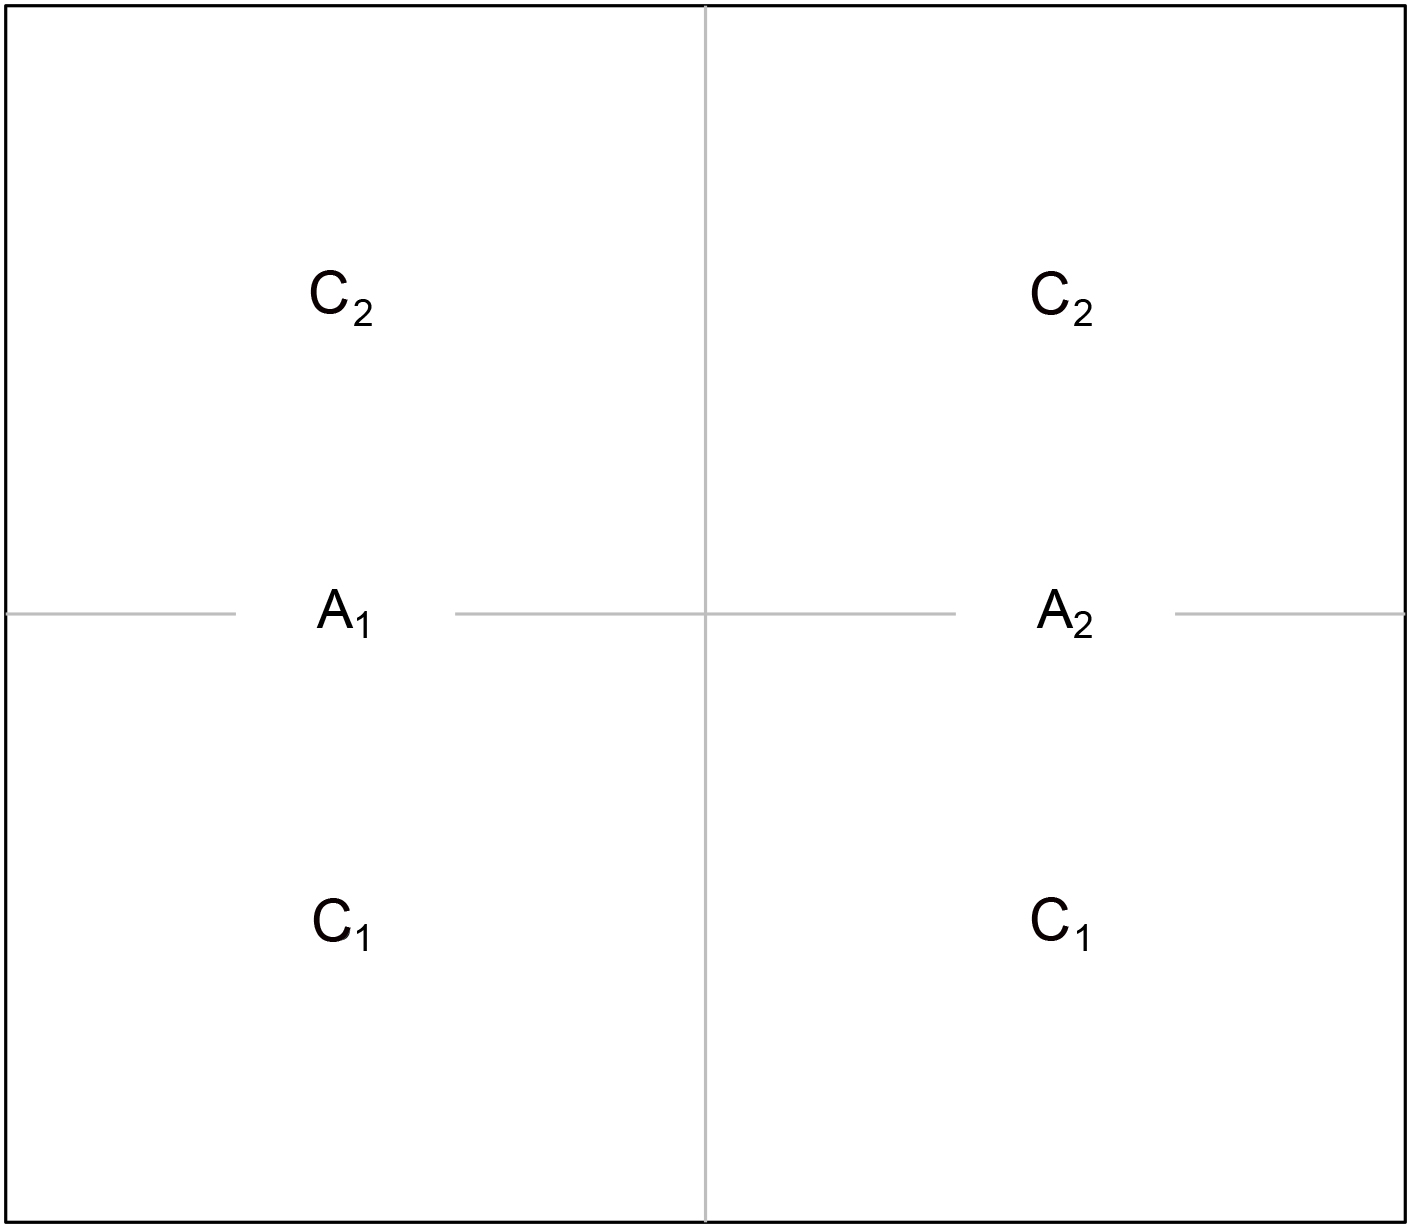
\includegraphics[trim= 0 0 0 0, clip,width=.45\textwidth]{split.jpg}\\
\caption{A split-plot design with whole-plot (factor $A$) and a split-plot (factor $C$).  I reserve (perhaps confusingly) factor $B$ for blocks and replicates.}
\label{fig:crsp}
\end{figure}


\subsection{CRD in Whole-Plots Design (CRSP)}
In \textit{simple split-plot designs}, the whole-plot levels are generally assigned to larger block units following a CRD framework and split-plot levels are  assigned to smaller portions of the whole-plot levels using a CRD.
\vspace{0.05in}

\noindent\textbf{Model:} \[Y_{ijk} = \mu + \alpha_i + \beta_{j(i)} + \gamma_k + (\alpha\beta)_{j(i)} + \varepsilon_{ijk} \hspace{0.2in} \left\{
                \begin{array}{ll}
                  i = 1,2,\dots,a\\
                  j = 1,2,\dots,b\\
                  k = 1,2,\dots,c
                \end{array}
              \right.\]

\noindent where $Y_{ijk}$ is the \textit{j}th whole-plot experimental unit for the \textit{k}th split-plot and the \textit{i}th whole-plot factor level, $\mu$ is the true grand mean, $\alpha_i$ is the \textit{i}th whole-plot level effect from \textit{A}, $\beta_j$ is the $j$th whole-plot experimental unit, $\gamma_{k(i)}$ is the \textit{k}th split-plot level in $C$ in the $i$th whole-plot level in $A$, and $\varepsilon_{ijk}$ is the error from the \textit{j}th whole-plot experimental unit, in the \textit{k}th split-plot level, in the \textit{i}th whole-plot level.
\vspace{0.05in}

\noindent \textbf{H$_0$:}
\begin{itemize}
\item $A$: $\mu_1 = \mu_2 = \dots = \mu_a$.
\item $C$: $\mu_1 = \mu_2 = \dots = \mu_c$.
\item \textit{A:C}: all $(\alpha\gamma)_{ik} = 0$.
\end{itemize}
\vspace{0.1in}

\noindent \textbf{Assumptions:} $\varepsilon_{ijk} \sim N(0, \sigma^2)$,  \hspace{0.1in} $\beta_j \sim N(0, \sigma^2_B)$, \hspace{0.1in} $\beta_j \perp \varepsilon_{ijk}$, \hspace{0.1in} $(\alpha\beta)_{ij} = 0$
\vspace{0.1in}

\begin{tcolorbox}[colback=yellow!50!red!25!white,colbacktitle=yellow!50!red,colframe=black!75!white,title=\textbf{R:} CRSP]
\textbf{Framework:}\\
\vspace{-.2in}
\begin{knitrout}
\definecolor{shadecolor}{rgb}{0.969, 0.969, 0.969}\color{fgcolor}\begin{kframe}
\begin{alltt}
\hlkwd{summary}\hldef{(}\hlkwd{aov}\hldef{(Y} \hlopt{~} \hldef{A} \hlopt{*} \hldef{C} \hlopt{+} \hlkwd{Error}\hldef{(B} \hlopt{%in%} \hldef{C)))}
\end{alltt}
\end{kframe}
\end{knitrout}
\texttt{Y} = response variable, \texttt{A} is the whole-plot factor, \texttt{C} is the split-plot factor and \texttt{B} defines the whole-plot experimental unit.
\vspace{0.1in}
\par\noindent\rule{.9\textwidth}{0.4pt}

\textbf{Example 1} From \citep[][pg 113-119]{litt2007}. To assess the effect of processing approaches and silicon chip position on electrical resistance, twelve silicon wafers were randomly selected from a lot and were randomly assigned to four different processing modes. Resistance on the chips was measured in four different positions (four different chips) on each wafer. The whole-plot experimental units for process are the wafers. The split-plot experimental units for position are individual chips.  This a simple split plot design (no blocking is used)
\vspace{-.1in}
\begin{knitrout}
\definecolor{shadecolor}{rgb}{0.969, 0.969, 0.969}\color{fgcolor}\begin{kframe}
\begin{alltt}
\hlkwd{library}\hldef{(asbio);} \hlkwd{data}\hldef{(Semiconductor)}
\hlkwd{summary}\hldef{(}\hlkwd{aov}\hldef{(Resistance} \hlopt{~} \hldef{Process} \hlopt{*} \hldef{Chip} \hlopt{+} \hlkwd{Error}\hldef{(Wafer} \hlopt{%in%} \hldef{Process),}
            \hlkwc{data} \hldef{= Semiconductor))}
\end{alltt}
\end{kframe}
\end{knitrout}


\textbf{Example 2} From \citep[][pg 309-315]{lawson}.  To measure the drivers of cookie diameter, twelve batches of chocolate chip cookies were produced that varied with with respect to shortening amount (measured as a percentage), baking temperature, and tray temperature.  Shortening was more difficult vary and was used as a whole plot factor within which baking and tray types were assigned.  Thus, the design had two split plot factors (baking temperatures and tray temperatures) applied within each whole plot level (shortening levels) using a CRD.
\vspace{-.1in}
\begin{knitrout}
\definecolor{shadecolor}{rgb}{0.969, 0.969, 0.969}\color{fgcolor}\begin{kframe}
\begin{alltt}
\hlkwd{library}\hldef{(daewr);} \hlkwd{data}\hldef{(splitPdes);} \hlkwd{library}\hldef{(GAD)}
\hldef{Short} \hlkwb{<-} \hlkwd{as.fixed}\hldef{(splitPdes}\hlopt{$}\hldef{short)}
\hldef{Batch} \hlkwb{<-} \hlkwd{as.random}\hldef{(splitPdes}\hlopt{$}\hldef{batch)}
\hldef{BakeT} \hlkwb{<-} \hlkwd{as.fixed}\hldef{(splitPdes}\hlopt{$}\hldef{bakeT)}
\hldef{TrayT} \hlkwb{<-} \hlkwd{as.fixed}\hldef{(splitPdes}\hlopt{$}\hldef{trayT)}

\hldef{model} \hlkwb{<-} \hlkwd{aov}\hldef{(y} \hlopt{~} \hldef{Short} \hlopt{+} \hldef{Short}\hlopt{%in%}\hldef{Batch} \hlopt{+} \hldef{BakeT} \hlopt{+} \hldef{TrayT} \hlopt{+} \hldef{Short}\hlopt{*}\hldef{BakeT} \hlopt{+}
               \hldef{Short}\hlopt{*}\hldef{TrayT} \hlopt{+} \hldef{BakeT}\hlopt{*}\hldef{TrayT} \hlopt{+} \hldef{Short}\hlopt{*}\hldef{BakeT}\hlopt{*}\hldef{TrayT,}
            \hlkwc{data} \hldef{= splitPdes)}
\hlkwd{gad}\hldef{(model)}
\end{alltt}
\end{kframe}
\end{knitrout}
\end{tcolorbox}
\par\noindent\rule{.9\textwidth}{0.4pt}

\subsection{CRSP with Mixed Models}
\noindent\textbf{Model:} \[Y_{ijk} = \mu + \alpha_i + \gamma_{k(i)} + \beta_j + (\alpha\gamma)_{k(i)} + \varepsilon_{ijk} \hspace{0.2in} \left\{
                \begin{array}{ll}
                  i = 1,2,\dots,a\\
                  j = 1,2,\dots,b\\
                  k = 1,2,\dots,c
                \end{array}
              \right.\]

\noindent where $Y_{ijk}$ is the \textit{j}th response for the \textit{k}th split-plot and the \textit{i}th whole-plot factor level, $\mu$ is the true grand mean, $\alpha_i$ is the \textit{i}th whole-plot level effect from \textit{A}, $\beta_j$ is the $j$th whole-plot experimental unit, considered as a random effect, $\gamma_{k(i)}$ is the \textit{k}th split-plot level in $C$ in the $i$th whole-plot level in $A$, and $\varepsilon_{ijk}$ is the error from the \textit{j}th whole-plot experimental unit, in the \textit{k}th split-plot level, in the \textit{i}th whole-plot level. \\
\vspace{0.05in}

\noindent \textbf{H$_0$:}
\begin{itemize}
\item $A$: $\mu_1 = \mu_2 = \dots = \mu_a$.
\item $C$: $\mu_1 = \mu_2 = \dots = \mu_c$.
\item \textit{A:C}: all $(\alpha\gamma)_{ik} = 0$.
\item \textit{A:B}: $\sigma^2_{AB} = 0$.
\end{itemize}
\vspace{0.1in}

\noindent \textbf{Assumptions:} $\varepsilon_{ijk} \sim N(0, \sigma^2)$, \hspace{0.1in} $\beta_{j} \sim N(0, \sigma_B^2)$, \hspace{0.1in} $\beta_{j} \perp , \varepsilon_{ijk}$, \hspace{0.1in} $(\alpha\beta)_{ij} = 0$
\vspace{0.1in}

\begin{tcolorbox}[colback=yellow!50!red!25!white,colbacktitle=yellow!50!red,colframe=black!75!white,title=\textbf{R:} CRSP with Mixed Models]
\textbf{Framework:}\\
\vspace{-.2in}
\begin{knitrout}
\definecolor{shadecolor}{rgb}{0.969, 0.969, 0.969}\color{fgcolor}\begin{kframe}
\begin{alltt}
\hlkwd{library}\hldef{(lme4);} \hlkwd{library}\hldef{(lmerTest)}
\hldef{model} \hlkwb{<-} \hlkwd{lmer}\hldef{(Y} \hlopt{~} \hldef{A} \hlopt{*} \hldef{C} \hlopt{+} \hldef{(}\hlnum{1}\hlopt{|}\hldef{B}\hlopt{%in%}\hldef{A))}
\hlkwd{anova}\hldef{(model)} \hlcom{# fixed effects}
\hlkwd{ranova}\hldef{(model)} \hlcom{# random effects}
\end{alltt}
\end{kframe}
\end{knitrout}
\texttt{Y} = response variable, \texttt{A} is the whole-plot factor, \texttt{C} is the split-plot factor and \texttt{B} defines the whole-plot experimental unit (a random effect).
\vspace{0.1in}
\par\noindent\rule{.9\textwidth}{0.4pt}

\textbf{Example:} From \citep[][pg 120-124]{litt2007}.  In the Semiconductor example, mode of processing and position of chips were fixed factors, while wafer is a random effect.

\vspace{-.1in}
\begin{knitrout}
\definecolor{shadecolor}{rgb}{0.969, 0.969, 0.969}\color{fgcolor}\begin{kframe}
\begin{alltt}
\hlkwd{library}\hldef{(asbio);} \hlkwd{data}\hldef{(Semiconductor)}
\hlkwd{library}\hldef{(lme4);} \hlkwd{library}\hldef{(lmerTest)}
\hldef{model} \hlkwb{<-} \hlkwd{lmer}\hldef{(Resistance} \hlopt{~} \hldef{Process} \hlopt{*} \hldef{Chip} \hlopt{+} \hldef{(}\hlnum{1}\hlopt{|}\hldef{Wafer}\hlopt{%in%}\hldef{Process),}
            \hlkwc{data} \hldef{= Semiconductor)}
\hlkwd{anova}\hldef{(model)} \hlcom{# fixed effects}
\hlkwd{ranova}\hldef{(model)} \hlcom{# random effects}
\end{alltt}
\end{kframe}
\end{knitrout}
\end{tcolorbox}
\par\noindent\rule{.9\textwidth}{0.4pt}



\subsection{RBD in Whole-Plots Design (RBSP)}
This blocked design has also been called the \textit{usual} split-plot design \citep{milliken}.  In this case, whole-plot levels are explicitly assigned within blocks (Fig. \ref{fig:srbp}).

\begin{figure}[H]
\centering
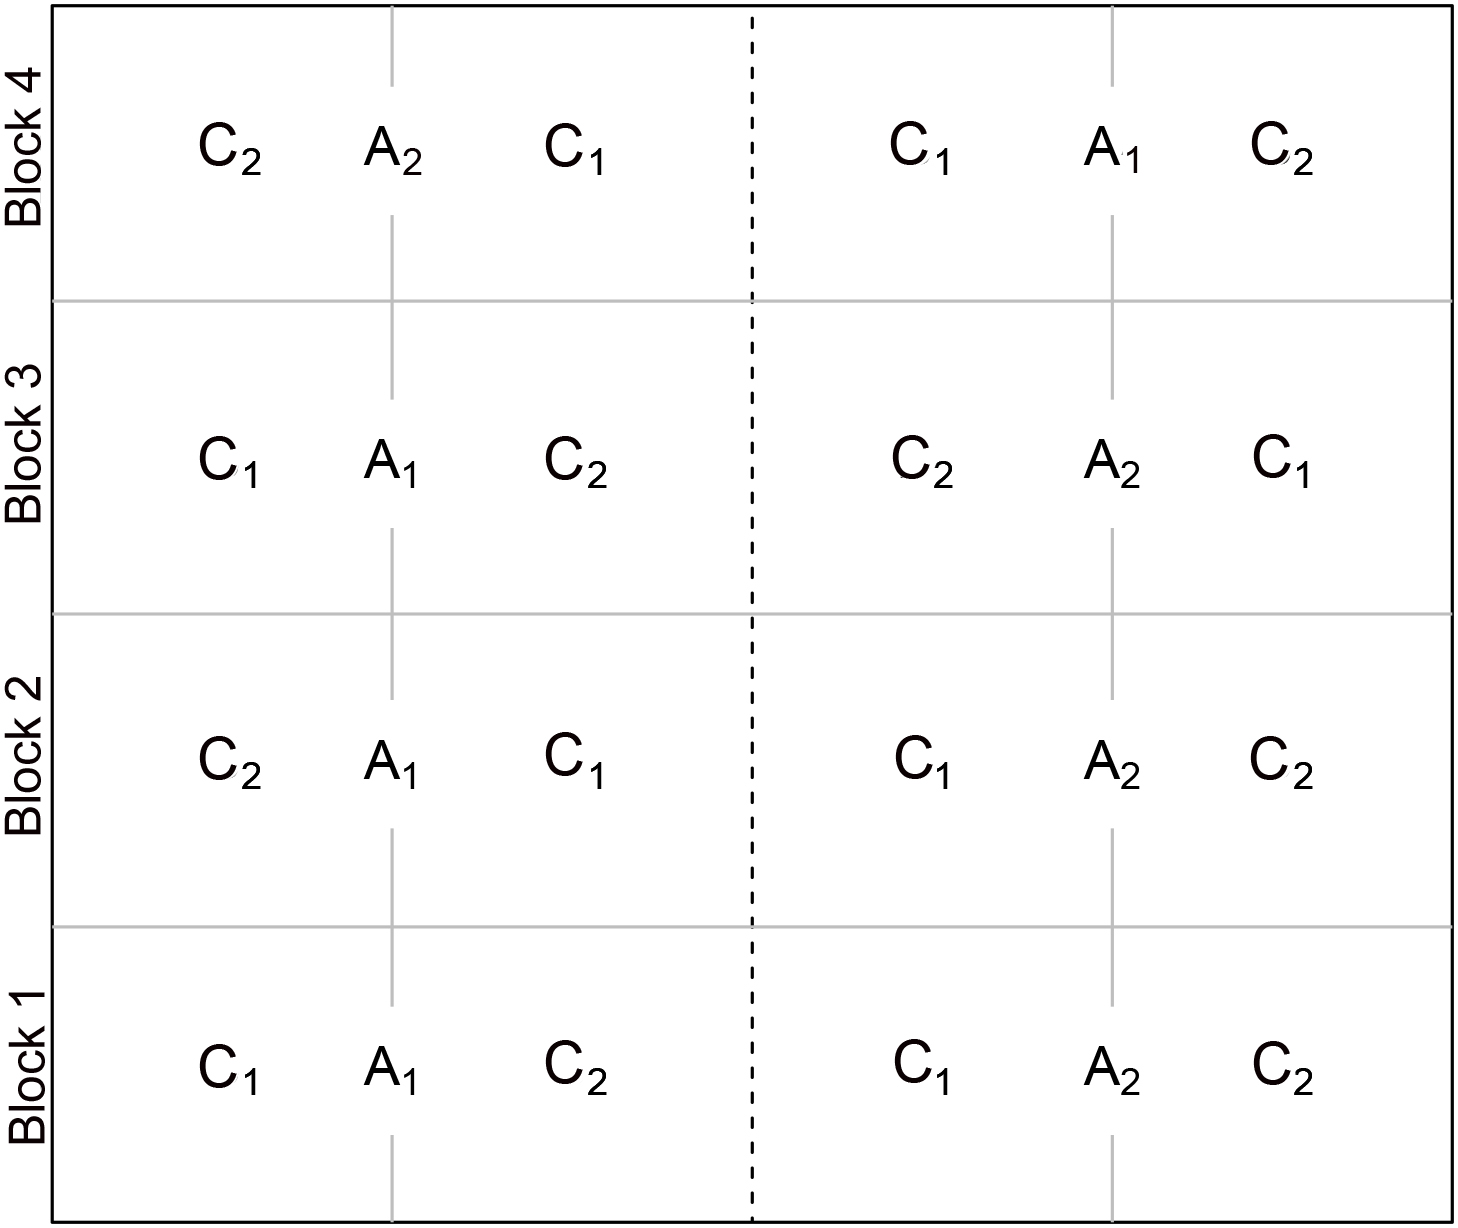
\includegraphics[trim= 0 0 0 0, clip,width=.45\textwidth]{SPRB.jpg}\\
\caption{A RBSP design with a whole-plot (factor $A$) and a split-plot (factor $C$). whole-plot levels are replicated at each of four blocks (factor $B$).  }
\label{fig:srbp}
\end{figure}

\noindent\textbf{Model:} \[Y_{ijk} = \mu + \alpha_i + \gamma_{k(i)} + \beta_j + (\alpha\gamma)_{k(i)} + \varepsilon_{ijk} \hspace{0.2in} \left\{
                \begin{array}{ll}
                  i = 1,2,\dots,a\\
                  j = 1,2,\dots,b\\
                  k = 1,2,\dots,c
                \end{array}
              \right.\]

\noindent where $Y_{ijk}$ is the response from the \textit{j}th block for the \textit{k}th split-plot and the \textit{i}th whole-plot factor level, $\mu$ is the true grand mean, $\alpha_i$ is the \textit{i}th whole-plot level effect from \textit{A}, $\beta_j$ is the $j$th blocking level, $\gamma_{k(i)}$ is the \textit{k}th split-plot level in $C$ in the $i$th whole-plot level in $A$, and $\varepsilon_{ijk}$ is the error from the \textit{j}th whole-plot experimental unit, in the \textit{k}th split-plot level, in the \textit{i}th whole-plot level. \\
\vspace{0.05in}

\noindent \textbf{H$_0$:}
\begin{itemize}
\item $A$: $\mu_1 = \mu_2 = \dots = \mu_a$.
\item $C$: $\mu_1 = \mu_2 = \dots = \mu_c$.
\item \textit{A:C}: all $(\alpha\gamma)_{ik} = 0$.
\end{itemize}
\vspace{0.1in}

\noindent \textbf{Assumptions:} $\varepsilon_{ijk} \sim N(0, \sigma^2)$, \hspace{0.1in} $(\alpha\beta)_{ij} = 0$
\vspace{0.1in}

\begin{tcolorbox}[colback=yellow!50!red!25!white,colbacktitle=yellow!50!red,colframe=black!75!white,title=\textbf{R:} RBSP]
\textbf{Framework:}\\
\vspace{-.2in}
\begin{knitrout}
\definecolor{shadecolor}{rgb}{0.969, 0.969, 0.969}\color{fgcolor}\begin{kframe}
\begin{alltt}
\hlkwd{summary}\hldef{(}\hlkwd{aov}\hldef{(Y} \hlopt{~} \hldef{A} \hlopt{*} \hldef{C} \hlopt{+} \hlkwd{Error}\hldef{(B}\hlopt{/}\hldef{A)))}
\end{alltt}
\end{kframe}
\end{knitrout}
\texttt{Y} = response variable, \texttt{A} is the whole-plot factor, \texttt{C} is the split-plot factor, and \texttt{B} defines the blocking variable.
\vspace{0.1in}
\par\noindent\rule{.9\textwidth}{0.4pt}

\textbf{Example:} \citet{snedecor} conducted an experiment to measure how different varieties of alfalfa responded to the last cutting day of the previous year. There were two factors: 1) variety of alfalfa (three varieties were planted in each of three randomly chosen whole-plots), and 2) the date of last cutting (Sept 1, Sept. 20, or Oct. 7). The dates were randomly chosen split-plots within the whole-plots. Replication was accomplished using six blocks of fields.
\vspace{-.1in}
\begin{knitrout}
\definecolor{shadecolor}{rgb}{0.969, 0.969, 0.969}\color{fgcolor}\begin{kframe}
\begin{alltt}
\hlkwd{library}\hldef{(asbio);} \hlkwd{data}\hldef{(alfalfa.split.plot)}
\hlkwd{summary}\hldef{(}\hlkwd{aov}\hldef{(yield} \hlopt{~} \hldef{variety} \hlopt{*} \hldef{cut.time} \hlopt{+} \hlkwd{Error}\hldef{(block}\hlopt{/}\hldef{variety),}
            \hlkwc{data} \hldef{= alfalfa.split.plot))}
\end{alltt}
\end{kframe}
\end{knitrout}
\end{tcolorbox}
\par\noindent\rule{.9\textwidth}{0.4pt}


\subsection{RBSP with Mixed Models}

\noindent\textbf{Model:} \[Y_{ijk} = \mu + \alpha_i + \gamma_{k(i)} + \beta_j + (\alpha\gamma)_{k(i)} + \varepsilon_{ijk} \hspace{0.2in} \left\{
                \begin{array}{ll}
                  i = 1,2,\dots,a\\
                  j = 1,2,\dots,b\\
                  k = 1,2,\dots,c
                \end{array}
              \right.\]

\noindent where $Y_{ijk}$ is the response from the \textit{j}th block for the \textit{k}th split-plot and the \textit{i}th whole-plot factor level, $\mu$ is the true grand mean, $\alpha_i$ is the \textit{i}th whole-plot level effect from \textit{A}, $\beta_j$ is the $j$th blocking level, $\gamma_{k(i)}$ is the \textit{k}th split-plot level in $C$ in the $i$th whole-plot level in $A$, and $\varepsilon_{ijk}$ is the error from the \textit{j}th whole-plot experimental unit, in the \textit{k}th split-plot level, in the \textit{i}th whole-plot level. \\
\vspace{0.05in}\\

\noindent \textbf{H$_0$:}
\begin{itemize}
\item $A$: $\mu_1 = \mu_2 = \dots = \mu_A$.
\item $C$: $\mu_1 = \mu_2 = \dots = \mu_C$.
\item \textit{A:C}: all $(\alpha\gamma)_{ik} = 0$.
\item \textit{A:B}: $\sigma^2_{AB} = 0$.
\end{itemize}
\vspace{0.1in}

\noindent \textbf{Assumptions:} $\varepsilon_{ijk} \sim N(0, \sigma^2)$, \hspace{0.1in}$\beta_{j} \sim N(0, \sigma_B^2)$, \hspace{0.1in} $\beta_{j} \perp , \varepsilon_{ijk}$, \hspace{0.1in} $(\alpha\beta)_{ij} = 0.$
\vspace{0.1in}

\begin{tcolorbox}[colback=yellow!50!red!25!white,colbacktitle=yellow!50!red,colframe=black!75!white,title=\textbf{R:} RBSP with Mixed Models]
\textbf{Framework:}\\
\vspace{-.2in}
\begin{knitrout}
\definecolor{shadecolor}{rgb}{0.969, 0.969, 0.969}\color{fgcolor}\begin{kframe}
\begin{alltt}
\hlkwd{library}\hldef{(lme4);} \hlkwd{library}\hldef{(lmerTest)}
\hldef{model} \hlkwb{<-} \hlkwd{lmer}\hldef{(Y} \hlopt{~} \hldef{A} \hlopt{*} \hldef{C} \hlopt{+} \hldef{(}\hlnum{1}\hlopt{|}\hldef{B)} \hlopt{+} \hldef{(}\hlnum{1}\hlopt{|}\hldef{B}\hlopt{/}\hldef{A))}
\hlkwd{anova}\hldef{(model)} \hlcom{# fixed effects}
\hlkwd{ranova}\hldef{(model)} \hlcom{# random effects}
\end{alltt}
\end{kframe}
\end{knitrout}
\texttt{Y} = response variable, \texttt{A} is the whole-plot factor, \texttt{C} is the split-plot factor, and \texttt{B} defines the blocking variable.
\vspace{0.1in}
\par\noindent\rule{.9\textwidth}{0.4pt}

\textbf{Example:} In the alfalfa split-plot experiment the blocking variable is a random effect.
\begin{knitrout}
\definecolor{shadecolor}{rgb}{0.969, 0.969, 0.969}\color{fgcolor}\begin{kframe}
\begin{alltt}
\hlkwd{library}\hldef{(asbio);} \hlkwd{data}\hldef{(alfalfa.split.plot)}
\hlkwd{library}\hldef{(nlme);} \hlkwd{library}\hldef{(lmerTest)}
\hldef{model} \hlkwb{<-} \hlkwd{lmer}\hldef{(yield} \hlopt{~} \hldef{variety} \hlopt{*} \hldef{cut.time} \hlopt{+} \hldef{(}\hlnum{1}\hlopt{|}\hldef{block}\hlopt{/}\hldef{variety),}
          \hlkwc{data} \hldef{= alfalfa.split.plot)}
\hlkwd{anova}\hldef{(model)}
\hlkwd{ranova}\hldef{(model)}
\end{alltt}
\end{kframe}
\end{knitrout}
\end{tcolorbox}

\par\noindent\rule{.9\textwidth}{0.4pt}
\subsection{Split-Split-Plot Design}
A \textit{split-split-plot design} will have two levels of split-plot nesting: $D$ (split-split-plots) are split-plots within $C$ (split-plots), and levels in $B$ are split-plots within $A$ (whole-plots) (Fig. \ref{fig:ssp}). $B$ is a blocking or replicate factor depending on the experimental design.

\begin{figure}[H]
\centering
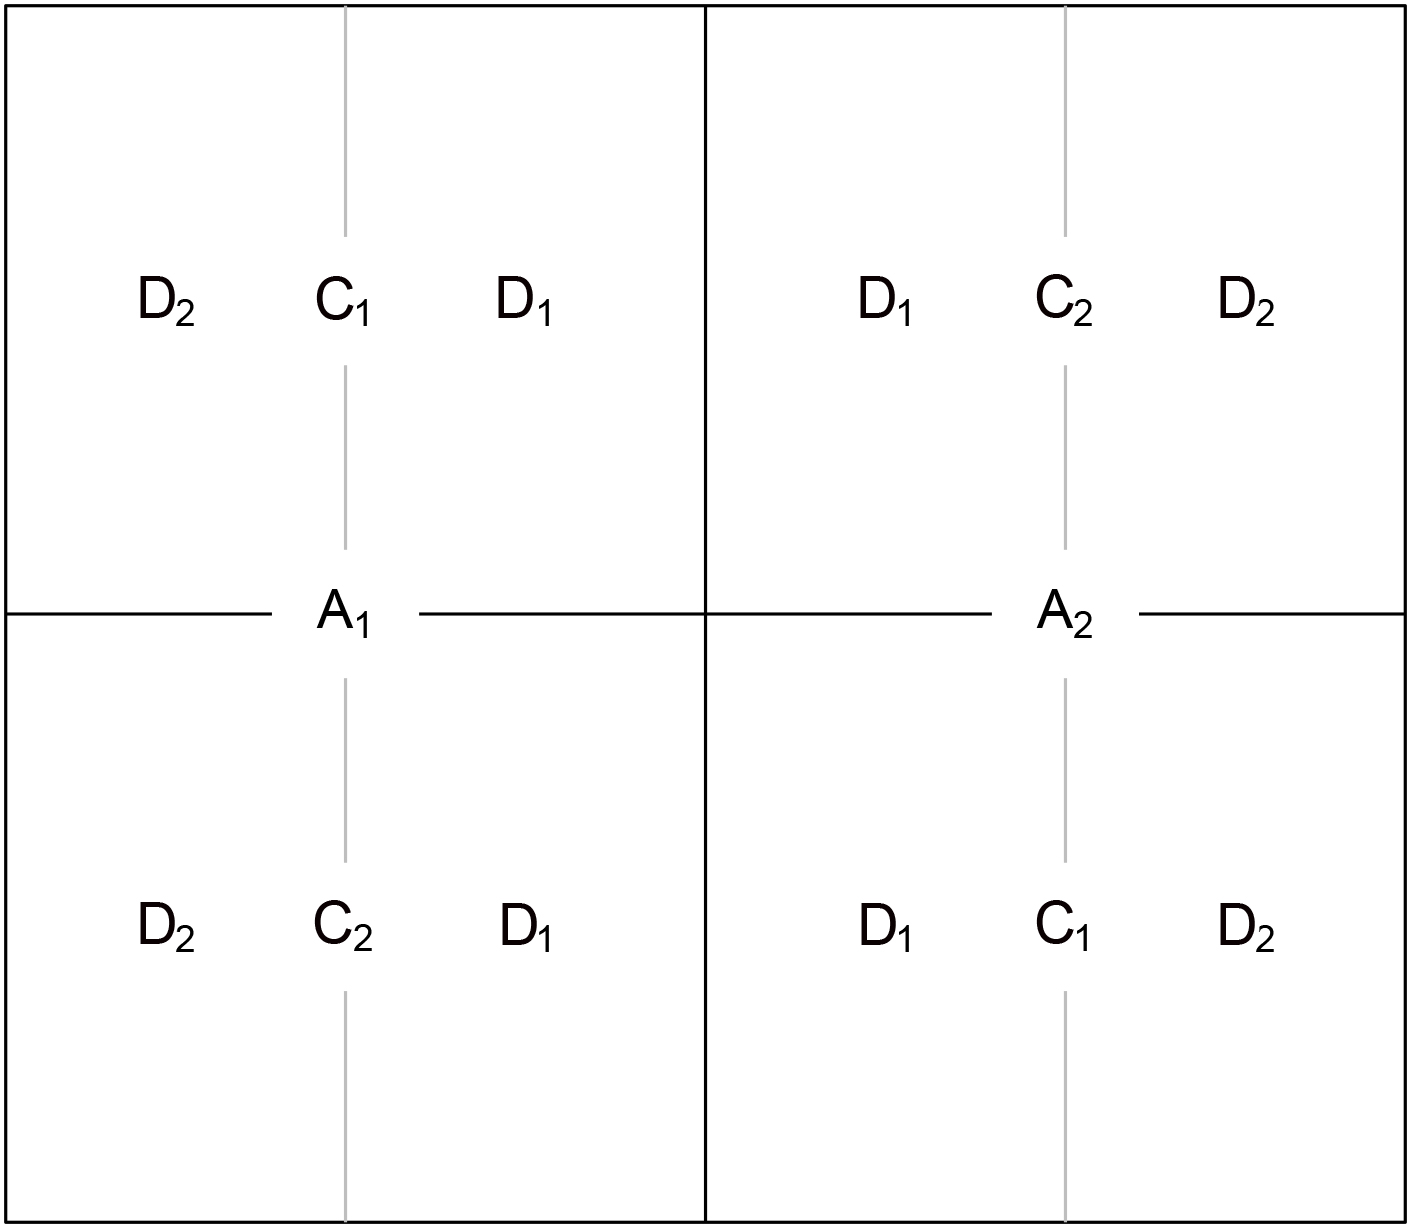
\includegraphics[trim= 0 0 0 0, clip,width=.45\textwidth]{split_split.jpg}\\
\caption{A split-split-plot design.  $A$ is the whole-plot factor, $C$ is the split-plot factor, and $D$ is the split-split-plot factor. The factor $B$, not shown, would define blocking (RBSP) or replication (CRSP). }
\label{fig:ssp}
\end{figure}

\noindent\textbf{Model:} \[Y_{ijkl} = \mu + \alpha_i + \gamma_{k(i)} +  \delta_{l(k(i))} + \beta_j + (\alpha\gamma)_{k(i)} + (\alpha\gamma)_{k(i)} + \varepsilon_{ijk} \hspace{0.2in} \left\{
                \begin{array}{ll}
                  i = 1,2,\dots,a\\
                  j = 1,2,\dots,b\\
                  k = 1,2,\dots,c\\
                  l = 1,2,\dots,d\\
                \end{array}
              \right.\]

\noindent where $Y_{ijkl}$ is the response from the \textit{j}th block for the \textit{l}th split-split-plot, for the \textit{k}th split-plot and the \textit{i}th whole-plot factor level, $\mu$ is the true grand mean, $\alpha_i$ is the \textit{i}th whole-plot level effect from \textit{A}, $\beta_j$ is the $j$th blocking level, $\delta_{l(k(i))}$ is the \textit{k}th split-plot level in $D$, in the $k$th split-plot level in $C$ in the $i$th whole-plot level in $A$, $\gamma_{k(i)}$ is the \textit{k}th split-plot level in $C$ in the $i$th whole-plot level in $A$, and $\varepsilon_{ijkl}$ is the error term. \\
\vspace{0.05in}

\noindent \textbf{Assumptions:} $\varepsilon_{ijk} \sim N(0, \sigma^2)$, \hspace{0.1in}$\beta_{j} \sim N(0, \sigma_B^2)$, \hspace{0.1in} $\beta_{j} \perp , \varepsilon_{ijk}$, \hspace{0.1in} $(\alpha\beta)_{ij} = 0$

\noindent \textbf{H$_0$:}
\begin{itemize}
\item $A$: $\mu_1 = \mu_2 = \dots = \mu_a$.
\item $C$: $\mu_1 = \mu_2 = \dots = \mu_c$.
\item $D$: $\mu_1 = \mu_2 = \dots = \mu_d$.
\item \textit{A:C}: all $(\alpha\gamma)_{ik} = 0$.
\item \textit{A:D}: all $(\alpha\delta)_{ik} = 0$.
\item \textit{C:D}: all $(\gamma\delta)_{ik} = 0$.
\item \textit{A:C:D}: all $(\alpha\gamma\delta)_{ik} = 0$.
\end{itemize}
\vspace{0.1in}

\begin{tcolorbox}[colback=yellow!50!red!25!white,colbacktitle=yellow!50!red,colframe=black!75!white,title=\textbf{R:} Split-Split-Plot]
\textbf{Framework:}\\
\vspace{-.2in}
\begin{knitrout}
\definecolor{shadecolor}{rgb}{0.969, 0.969, 0.969}\color{fgcolor}\begin{kframe}
\begin{alltt}
\hlkwd{summary}\hldef{(}\hlkwd{aov}\hldef{(Y} \hlopt{~} \hldef{A} \hlopt{*} \hldef{C} \hlopt{*} \hldef{D} \hlopt{+} \hlkwd{Error}\hldef{(B}\hlopt{/}\hldef{A}\hlopt{/}\hldef{C)))}
\end{alltt}
\end{kframe}
\end{knitrout}
\texttt{Y} = response variable, \texttt{A} is the whole-plot factor, \texttt{C} is the split-plot factor, \texttt{D} is the split-split-plot factor, and \texttt{B} defines the blocking variable.
\vspace{0.1in}
\par\noindent\rule{.9\textwidth}{0.4pt}

\textbf{Example:} \citep{hoshmand}. An experiment in Michigan was conducted to determine the influence of plant density and hybrids on corn (\textit{Zea mays} L.) yield.  The experiment was replicated four times in a randomized complete block design, arranged in a split-split-plot format.
\begin{knitrout}
\definecolor{shadecolor}{rgb}{0.969, 0.969, 0.969}\color{fgcolor}\begin{kframe}
\begin{alltt}
\hldef{corn} \hlkwb{<-} \hlkwd{data.frame}\hldef{(}\hlkwc{yield}\hldef{=}  \hlkwd{c}\hldef{(}\hlnum{140}\hldef{,}\hlnum{145}\hldef{,}\hlnum{150}\hldef{,}\hlnum{138}\hldef{,}\hlnum{146}\hldef{,}\hlnum{149}\hldef{,}\hlnum{130}\hldef{,}\hlnum{150}\hldef{,}
                             \hlnum{146}\hldef{,}\hlnum{142}\hldef{,}\hlnum{147}\hldef{,}\hlnum{150}\hldef{,}\hlnum{136}\hldef{,}\hlnum{140}\hldef{,}\hlnum{145}\hldef{,}\hlnum{132}\hldef{,}
                             \hlnum{134}\hldef{,}\hlnum{138}\hldef{,}\hlnum{134}\hldef{,}\hlnum{136}\hldef{,}\hlnum{138}\hldef{,}\hlnum{138}\hldef{,}\hlnum{140}\hldef{,}\hlnum{142}\hldef{,}
                             \hlnum{142}\hldef{,}\hlnum{146}\hldef{,}\hlnum{148}\hldef{,}\hlnum{132}\hldef{,}\hlnum{136}\hldef{,}\hlnum{140}\hldef{,}\hlnum{128}\hldef{,}\hlnum{140}\hldef{,}
                             \hlnum{142}\hldef{,}\hlnum{140}\hldef{,}\hlnum{141}\hldef{,}\hlnum{140}\hldef{,}\hlnum{132}\hldef{,}\hlnum{138}\hldef{,}\hlnum{140}\hldef{,}\hlnum{130}\hldef{,}
                             \hlnum{132}\hldef{,}\hlnum{134}\hldef{,}\hlnum{136}\hldef{,}\hlnum{130}\hldef{,}\hlnum{130}\hldef{,}\hlnum{134}\hldef{,}\hlnum{132}\hldef{,}\hlnum{136}\hldef{),}
        \hlkwc{reps} \hldef{=} \hlkwd{rep}\hldef{(}\hlkwd{rep}\hldef{(}\hlkwd{c}\hldef{(}\hlsng{"I"}\hldef{,}\hlsng{"II"}\hldef{,}\hlsng{"III"}\hldef{,}\hlsng{"IV"}\hldef{),} \hlkwc{each} \hldef{=} \hlnum{3}\hldef{),}\hlnum{4}\hldef{),}
        \hlkwc{density} \hldef{=} \hlkwd{rep}\hldef{(}\hlkwd{rep}\hldef{(}\hlkwd{c}\hldef{(}\hlsng{"12,000"}\hldef{,}\hlsng{"16,000"}\hldef{,} \hlsng{"20,000"}\hldef{),}\hlnum{4}\hldef{),}\hlnum{4}\hldef{),}
        \hlkwc{spacing} \hldef{=} \hlkwd{rep}\hldef{(}\hlkwd{c}\hldef{(}\hlsng{"12"}\hldef{,}\hlsng{"25"}\hldef{,}\hlsng{"12"}\hldef{,} \hlsng{"25"}\hldef{),} \hlkwc{each} \hldef{=} \hlnum{12}\hldef{),}
        \hlkwc{hybrid} \hldef{=} \hlkwd{rep}\hldef{(}\hlkwd{c}\hldef{(}\hlsng{"P3730"}\hldef{,} \hlsng{"B70XLH55"}\hldef{),} \hlkwc{each} \hldef{=} \hlnum{24}\hldef{))}

\hlkwd{summary}\hldef{(}\hlkwd{aov}\hldef{(yield} \hlopt{~} \hldef{hybrid} \hlopt{*} \hldef{spacing} \hlopt{*} \hldef{density} \hlopt{+}
              \hlkwd{Error}\hldef{(reps}\hlopt{/}\hldef{hybrid}\hlopt{/}\hldef{spacing),} \hlkwc{data} \hldef{= corn))}
\end{alltt}
\end{kframe}
\end{knitrout}
\end{tcolorbox}


\subsection{Strip Plot Designs}
\textit{Strip plots designs} can be used address situations when relatively large experimental units are required for each of two factors in an experiment. A strip plot will have a row and column structure \citep[see][]{lawson}. Let the number of columns equal the number of levels in factor $A$, and let the number of rows equal the number of levels in factor $B$. Levels in $A$ are randomly assigned to columns only (across all rows) in a CRD format, and levels in $B$ are assigned to rows only (across all columns) in a CRD format. Interestingly, the levels in $A$ serve as split-plots in $B$ and vice versa (Fig. \ref{fig:str}).  Compared to a factorial design, strip plots allow for greater precision in the measurement of interaction effects while sacrificing precision in the measurement of main effects.

\begin{figure}[H]
\centering
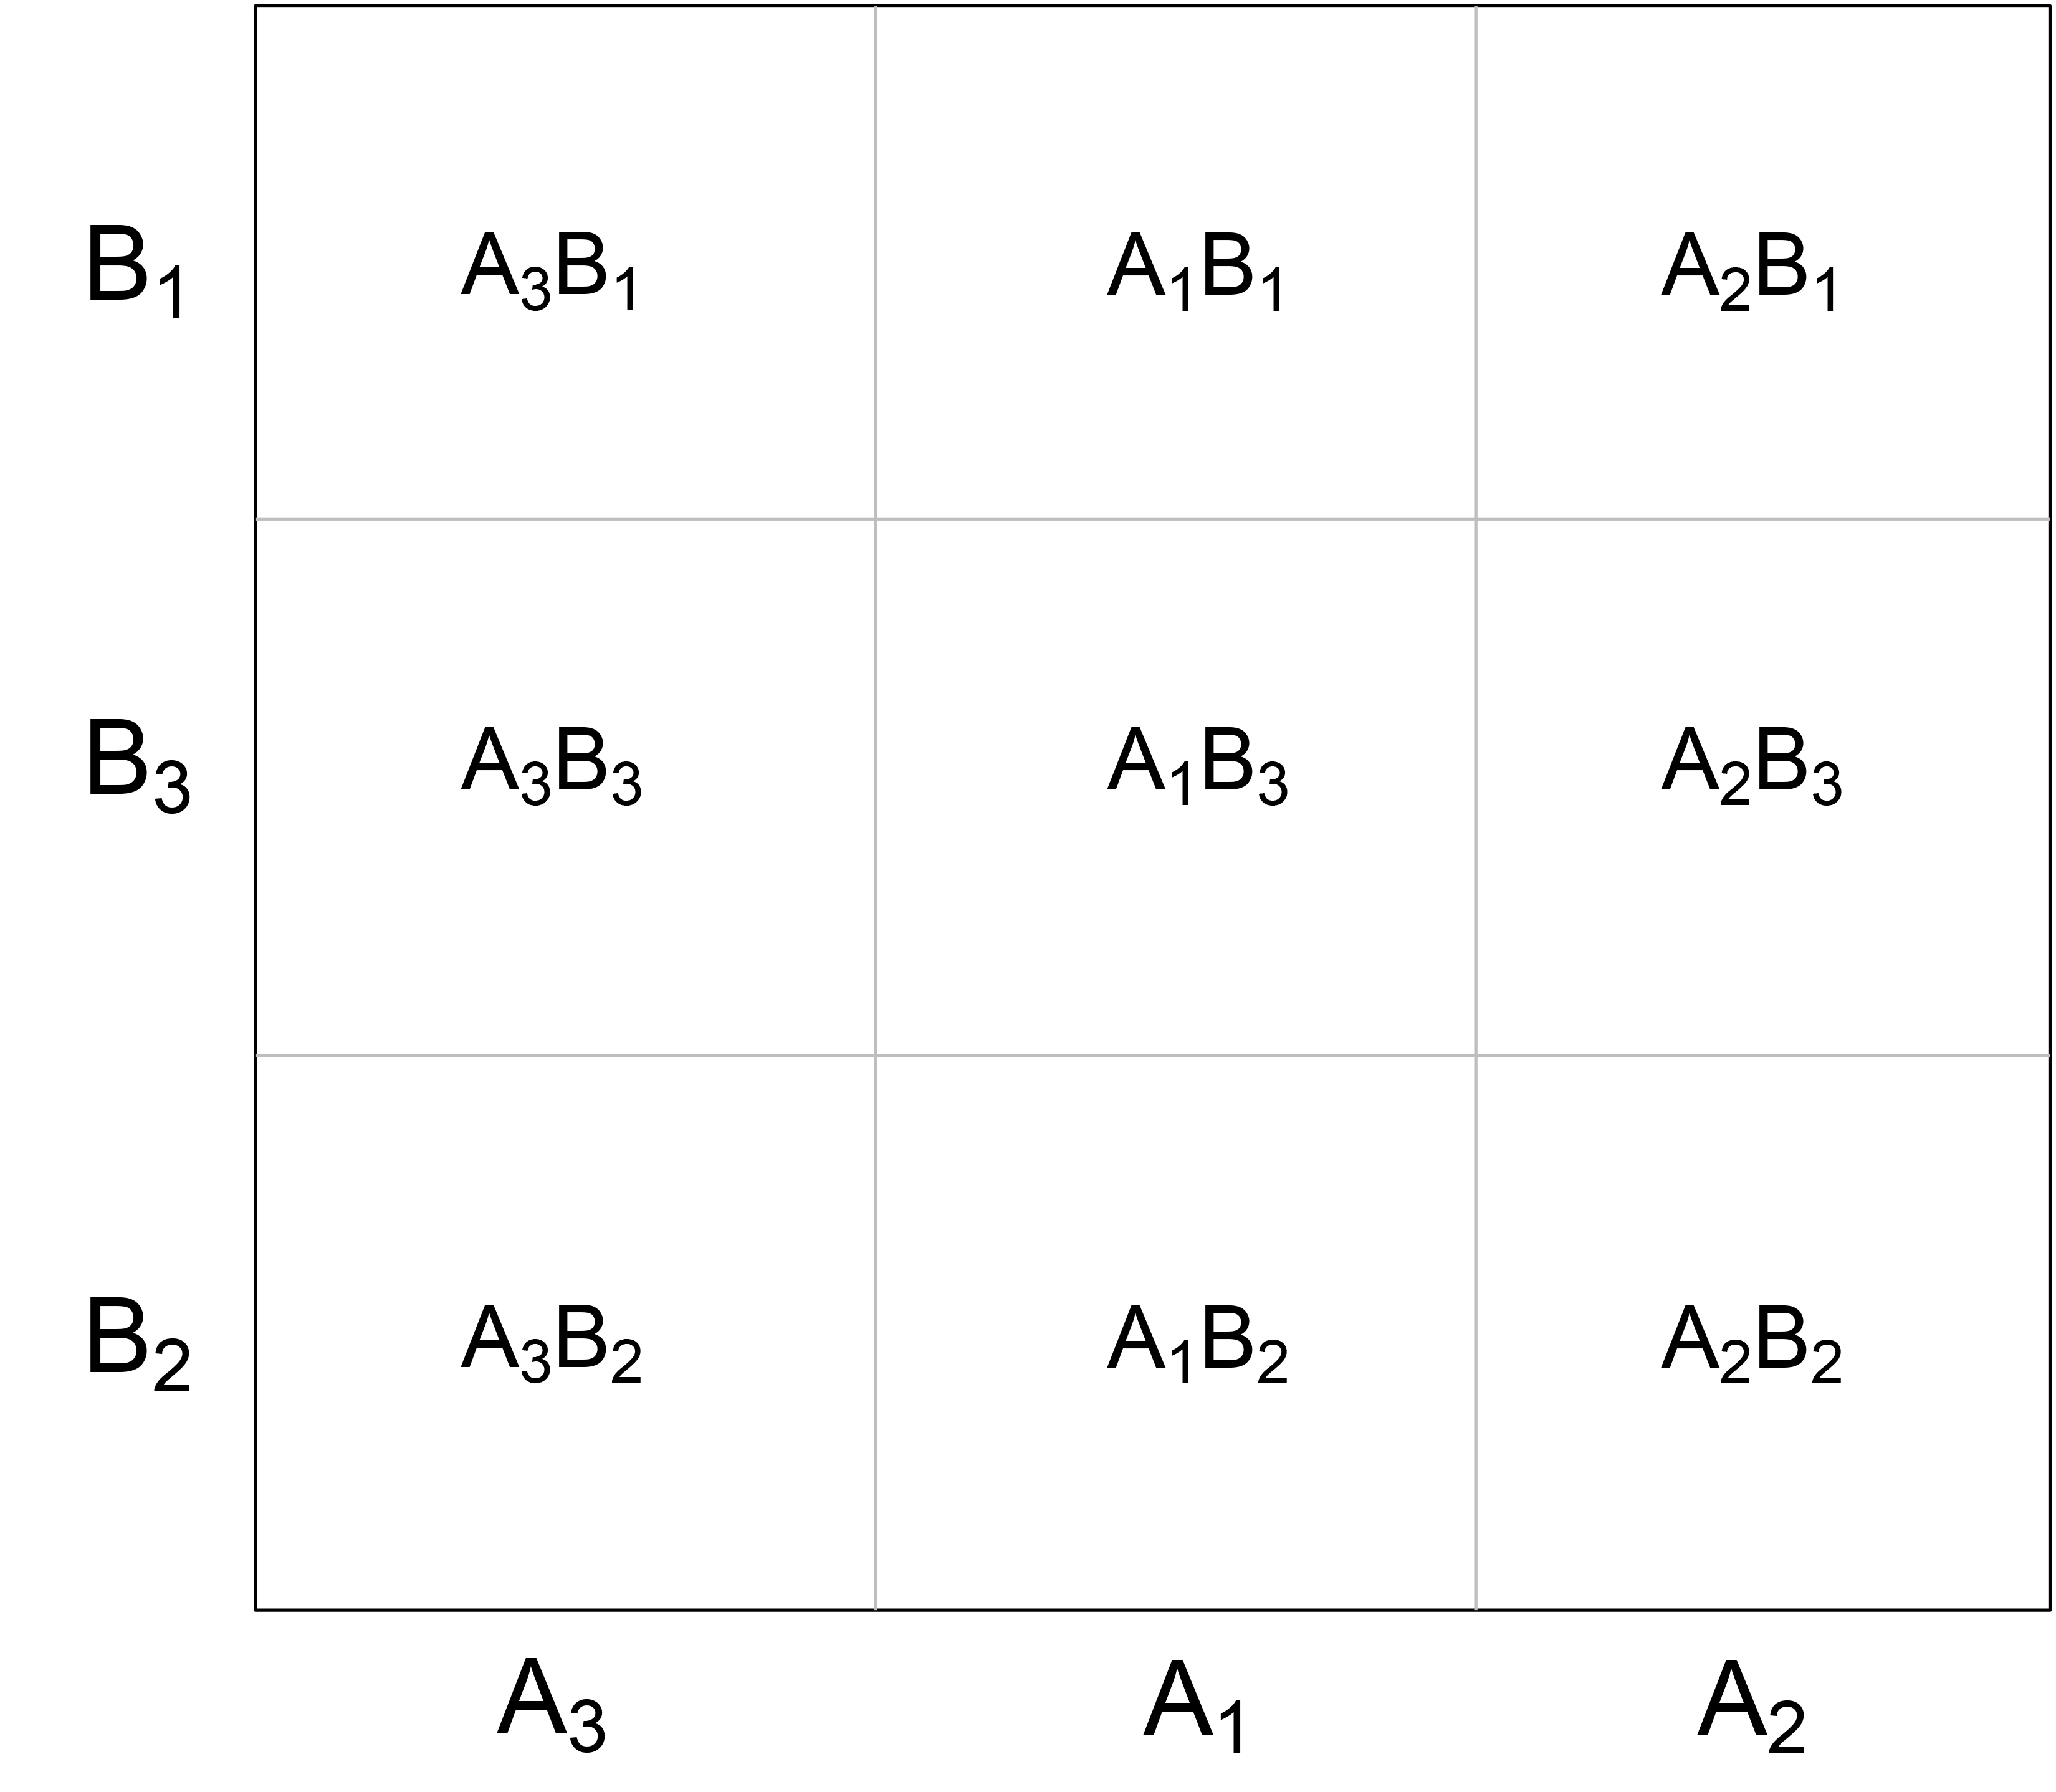
\includegraphics[trim= 0 0 0 0, clip,width=.45\textwidth]{strip.jpg}
\caption{A strip plot design with levels in $A$ assigned to columns and levels in $B$ assigned to rows.}
\label{fig:str}
\end{figure}

\newpage

\section{Repeated Measured Designs}
\subsection{Repeated Measures as an RCBD}
\vspace{0.05in}
\noindent As with an RCBD, the analysis reduces to a paired $t$-test given two levels in $A$ (Fig. \ref{fig:rm}).
\vspace{-.4in}
\begin{figure}[H]
\begin{knitrout}
\definecolor{shadecolor}{rgb}{0.969, 0.969, 0.969}\color{fgcolor}

{\centering 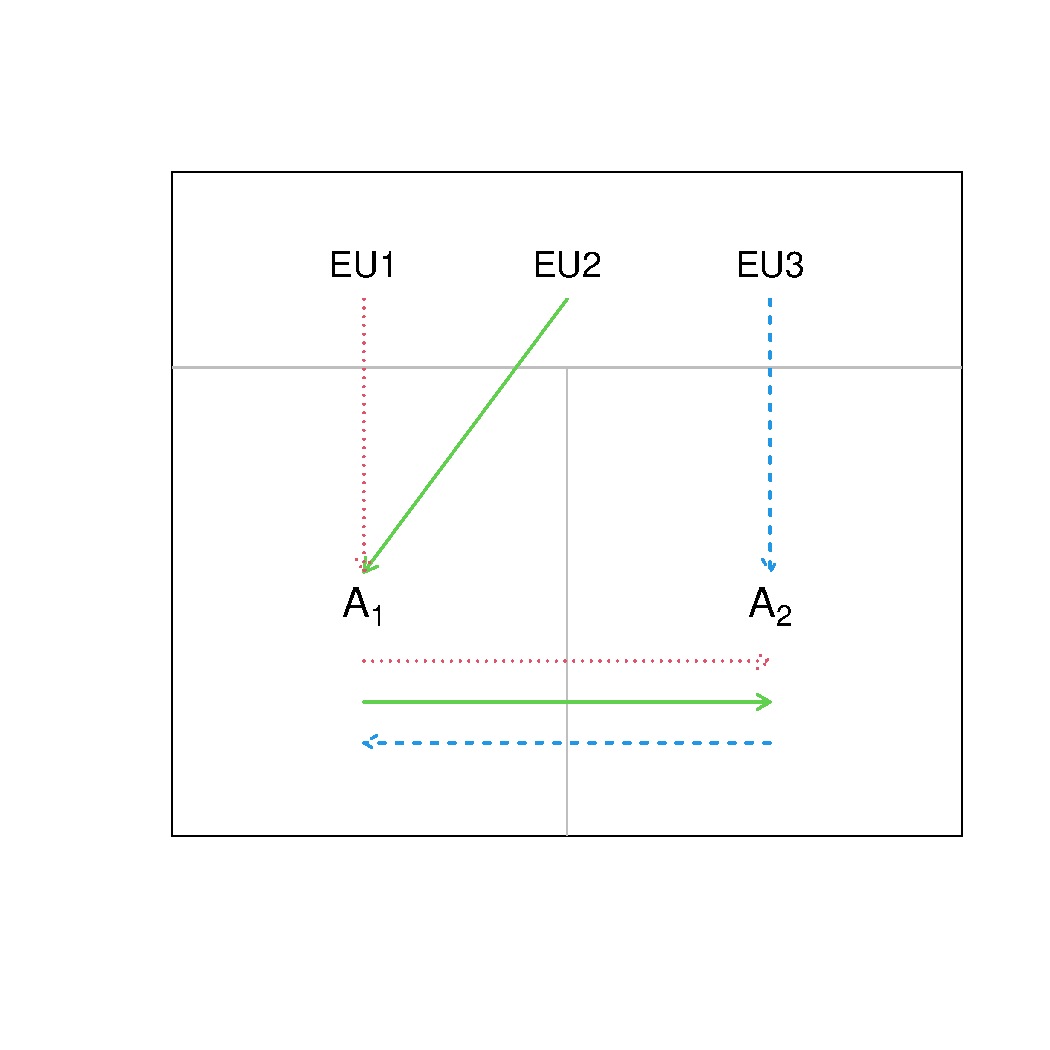
\includegraphics[width=.5\linewidth]{figure/minimal-unnamed-chunk-65-1} 

}


\end{knitrout}
\vspace{-.75in}
\caption{A matched pairs crossover design with three EUs and two treatments.}
\label{fig:rm}
\end{figure}
\vspace{0.05in}


\noindent \textbf{Model:} \[Y_{ij} = \mu + \alpha_i + \beta_j + \varepsilon_{ij} \hspace{0.2in} \left\{
\begin{array}{ll}
                  i = 1,2,\dots,a\\
                  j = 1,2,\dots,b\\
                  \end{array}
              \right.\]

\noindent where $Y_{ij}$ is the \textit{j}th (blocked by subject response) for the \textit{i}th factor level, $\mu$ is the true grand mean, $\alpha_i$ is the \textit{i}th factor level effect from \textit{A}, $\beta_j$ is the \textit{j}th factor level effect from blocking factor \textit{B}, and $\varepsilon_{ij}$ is the error the \textit{j}th block and the \textit{i}th factor level. \\
\vspace{0.05in}


\noindent \textbf{H$_0$:}
\begin{itemize}
\item $A$: $\mu_1 = \mu_2 = \dots = \mu_a$.
\item $B$: $\mu_1 = \mu_2 = \dots = \mu_b$.
\end{itemize}
\vspace{0.1in}

\noindent \textbf{Assumptions:} $\varepsilon_{ij} \sim N(0, \sigma^2)$.  The method assumes no carryover effects, i.e., it assumes time intervals are independent.
\vspace{0.1in}

\noindent \textbf{Robust Alternatives:}
\begin{small}
\begin{itemize}
\item Freidman test \citep{kruskal1952}, robust to non-normal errors, \textbf{R:} \texttt{freidman.test}\vspace{-.1in}
\item Agresti-Pendergrast test \citep{agresti1986}, more powerful than the Freidman test for most applications, \textbf{R:} \texttt{asbio::AP.test}
\end{itemize}
\end{small}
\vspace{0.1in}

\begin{tcolorbox}[colback=yellow!50!red!25!white,colbacktitle=yellow!50!red,colframe=black!75!white,title=\textbf{R:} Repeated Measures as an RCBD]

\textbf{Framework:}\\
\vspace{-.2in}
\begin{knitrout}
\definecolor{shadecolor}{rgb}{0.969, 0.969, 0.969}\color{fgcolor}\begin{kframe}
\begin{alltt}
\hlkwd{anova}\hldef{(}\hlkwd{lm}\hldef{(Y} \hlopt{~} \hldef{X} \hlopt{+} \hldef{B))}
\end{alltt}
\end{kframe}
\end{knitrout}
\vspace{-.1in}
or
\vspace{-.1in}
\begin{knitrout}
\definecolor{shadecolor}{rgb}{0.969, 0.969, 0.969}\color{fgcolor}\begin{kframe}
\begin{alltt}
\hlkwd{aov}\hldef{(Y} \hlopt{~} \hldef{A} \hlopt{+} \hldef{B)}
\end{alltt}
\end{kframe}
\end{knitrout}
\texttt{Y} = response variable, \texttt{A} = predictor, and \texttt{B} = blocking variable, e.g., subject.
\vspace{0.1in}
\par\noindent\rule{.9\textwidth}{0.4pt}

\textbf{Example:} From \citep[][pg 63]{litt2002}.  Five methods of irrigation were applied to a Valencia orange grove.  The trees in the grove were arranged in eight blocks.  Assignments of irrigation levels to trees within blocks was random.  Each irrigation method appears in all eight blocks, i.e., all blocks received all treatments, separated in time.
\vspace{-.1in}
\begin{knitrout}
\definecolor{shadecolor}{rgb}{0.969, 0.969, 0.969}\color{fgcolor}\begin{kframe}
\begin{alltt}
\hlkwd{library}\hldef{(asbio);} \hlkwd{data}\hldef{(fruit)}
\hlkwd{anova}\hldef{(}\hlkwd{lm}\hldef{(fruitwt} \hlopt{~} \hldef{irrig} \hlopt{+} \hldef{block,} \hlkwc{data} \hldef{= fruit))}
\end{alltt}
\end{kframe}
\end{knitrout}
\end{tcolorbox}
\par\noindent\rule{.9\textwidth}{0.4pt}

\subsection{Split-Plot in Time}
A block-less CRSP design can be implemented in a repeated measures context.  \citet[][pg. 502]{milliken} call this a \textit{split-plot in time}. \\

\noindent\textbf{Model:} \[Y_{ijk} = \mu + \alpha_i + \beta_{j} + \gamma_{k(i)} + (\alpha\gamma)_{k(i)} + \varepsilon_{ijk} \hspace{0.2in} \left\{
                \begin{array}{ll}
                  i = 1,2,\dots,a\\
                  j = 1,2,\dots,b\\
                  k = 1,2,\dots,c
                \end{array}
              \right.\]

\noindent where $Y_{ijk}$ is the \textit{j}th respondent (replicate or subject) observation for the \textit{k}th split-plot (time) levels and the \textit{i}th whole-plot level, $\mu$ is the true grand mean, $\alpha_i$ is the \textit{i}th whole-plot level effect from \textit{A}, $\beta_{j}$ is the $j$th subject (whole-plot experimental unit) level, $\gamma_{k(i)}$ is the \textit{k}th split-plot level in $B$ in the $i$th whole-plot level of $A$, and $\varepsilon_{ijk}$ is the error from the \textit{k}th subject, the \textit{j}th split-plot level, and the \textit{i}th whole-plot level. \\
\vspace{0.05in}

\noindent \textbf{H$_0$:}
\begin{itemize}
\item $A$: $\mu_1 = \mu_2 = \dots = \mu_a$.
\item $C$: $\mu_1 = \mu_2 = \dots = \mu_b$.
\item \textit{A:C}: all $(\alpha\gamma)_{ik} = 0$.
\end{itemize}
\vspace{0.1in}

\noindent \textbf{Assumptions:} $\varepsilon_{ijk} \sim N(0, \sigma^2)$, \hspace{0.1in}  $(\alpha\beta)_{ij} = 0$.  Correlation between measures on the same subject are assumed to be identical regardless of proximity in time, i.e., meets the Huyhn - Feldt condition.
\vspace{0.1in}

\begin{tcolorbox}[colback=yellow!50!red!25!white,colbacktitle=yellow!50!red,colframe=black!75!white,title=\textbf{R:} Split-Plot in Time]

\textbf{R framework:}\\
\vspace{-.2in}
\begin{knitrout}
\definecolor{shadecolor}{rgb}{0.969, 0.969, 0.969}\color{fgcolor}\begin{kframe}
\begin{alltt}
\hlkwd{summary}\hldef{(}\hlkwd{aov}\hldef{(Y} \hlopt{~} \hldef{A} \hlopt{*} \hldef{C} \hlopt{+} \hlkwd{Error}\hldef{(B} \hlopt{%in%} \hldef{A)))}
\end{alltt}
\end{kframe}
\end{knitrout}
where \texttt{Y} = response variable, \texttt{A} = whole-plot factor, \texttt{C} = slit plot time series, an ordered factor, and \texttt{B} = whole-plot experimental unit.
\vspace{0.1in}
\par\noindent\rule{.9\textwidth}{0.4pt}

\textbf{Example:} From \citep[][pg 506]{milliken}.
\vspace{-.1in}
\begin{knitrout}
\definecolor{shadecolor}{rgb}{0.969, 0.969, 0.969}\color{fgcolor}\begin{kframe}
\begin{alltt}
\hlkwd{library}\hldef{(asbio);} \hlkwd{data}\hldef{(heart)}
\hlkwd{summary}\hldef{(}\hlkwd{aov}\hldef{(rate} \hlopt{~} \hldef{drug} \hlopt{*} \hldef{time} \hlopt{+} \hlkwd{Error}\hldef{(subject} \hlopt{%in%} \hldef{drug),}
            \hlkwc{data} \hldef{= heart))}
\end{alltt}
\end{kframe}
\end{knitrout}
\end{tcolorbox}
\par\noindent\rule{.9\textwidth}{0.4pt}

\subsection{Repeated Measures ANOVA -- Analysis of Contrasts}
\textbf{Model:}

\noindent This is a multivariate general linear model that adjusts for violations of the H-F condition (asphericity) by reducing degrees of freedom, see \citep{aho2014}.
\vspace{0.1in}

\noindent \textbf{Assumptions:} In general, reflects assumptions and propensities of a multivariate general linear model.  For tests using non-adjusted degrees of freedom, we assume the H-F condition.
\vspace{0.1in}

\begin{tcolorbox}[colback=yellow!50!red!25!white,colbacktitle=yellow!50!red,colframe=black!75!white,title=\textbf{R:} Repeated Measures ANOVA]

\textbf{Framework:}\\
see below
\vspace{0.1in}
\par\noindent\rule{.9\textwidth}{0.4pt}

\textbf{Example:} From \citep[][pg 265]{litt2002}. The effect of two asthma drugs and a placebo were measured on 24 asthmatic patients. Each patient was randomly given each drug using an approach to minimize carry-over effects. Forced expiratory volume (FEV1), the volume of air that can be expired after taking a deep breath in one second, was measured hourly for eight hours following application of the drug. A baseline measure of FEV1 was also taken 11 hours before application of the treatment.
\vspace{-.1in}
\begin{knitrout}
\definecolor{shadecolor}{rgb}{0.969, 0.969, 0.969}\color{fgcolor}\begin{kframe}
\begin{alltt}
\hlkwd{library}\hldef{(car)}
\hlkwd{library}\hldef{(asbio);} \hlkwd{data}\hldef{(asthma)}
\hldef{m} \hlkwb{<-} \hlkwd{as.matrix}\hldef{(asthma[,}\hlnum{3}\hlopt{:}\hlnum{10}\hldef{])} \hlcom{# ignore baseline}
\hldef{asthma.lm} \hlkwb{<-} \hlkwd{lm}\hldef{(m} \hlopt{~} \hldef{DRUG,} \hlkwc{data} \hldef{= asthma)} \hlcom{# multivariate gen. lin. model}
\hldef{hr} \hlkwb{<-} \hlkwd{ordered}\hldef{(}\hlkwd{seq}\hldef{(}\hlnum{11}\hldef{,} \hlnum{18}\hldef{))}
\hlkwd{summary}\hldef{(}\hlkwd{Anova}\hldef{(asthma.lm,} \hlkwc{idesign} \hldef{=}\hlopt{~}\hldef{hr,} \hlkwc{idata} \hldef{=} \hlkwd{data.frame}\hldef{(hr)),}
        \hlkwc{multivariate} \hldef{=} \hlnum{FALSE}\hldef{)}
\end{alltt}
\end{kframe}
\end{knitrout}
\end{tcolorbox}
\par\noindent\rule{.9\textwidth}{0.4pt}

\subsection{Repeated Measures -- Mixed Model Approaches}
\noindent \textbf{Model:} \[Y_{ij} = \mu + \alpha_i + \beta_j + \varepsilon_{ij} \hspace{0.2in} \left\{
\begin{array}{ll}
                  i = 1,2,\dots,a\\
                  j = 1,2,\dots,n_i\\
                  \end{array}
              \right.\]

\noindent where $Y_{ij}$ is the \textit{j}th (blocked by subject response) for the \textit{i}th factor level, $\mu$ is the true grand mean, $\alpha_i$ is the \textit{i}th factor level effect from \textit{A}, $\beta_j$ is the \textit{j}th factor level effect from blocking factor (a random factor) \textit{B}, and $\varepsilon_{ij}$ is the error the \textit{j}th block and the \textit{i}th factor level. 

\vspace{0.05in}
\noindent This approach allows incredible flexibility when assessing and modelling autocorrelation of observations, see \citep{aho2014}.\\
\vspace{.05in}

\noindent \textbf{H$_0$:}
\begin{itemize}
\item $A$: $\mu_1 = \mu_2 = \dots = \mu_a$.
\item $B$: $\sigma^2_B = 0$\\
\end{itemize}
\vspace{0.05in}

\noindent \textbf{Assumptions:}
Assumptions can vary greatly with model specifications and designs. In general, we have: $\varepsilon_{ij} \sim N(0, \sigma^2)$, \hspace{0.1in} $\beta_{j} \sim N(0, \sigma_B^2)$, \hspace{0.1in} $\beta_{j} \perp \varepsilon_{ij}.$

\vspace{0.1in}

\paragraph{Covariance Structures:}
$Y_{ij}$'s are only assumed to be independent if they are from different random factor levels. Observations from the same factor level will have covariance $\sigma^2_B$. These relations can be considered in the context of the variance covariance matrix of $Y$.  Consider a model with a single random factor, $B$, that has two levels, and two observations for each level. The variance-covariance structure would be:
\[\boldsymbol{\sigma^2_Y} = \left[
 \begin{matrix}
  \sigma^2_Y & \sigma^2_B & 0 & 0 \\
  \sigma^2_B & \sigma^2_Y & 0 & 0 \\
  0 & 0 & \sigma^Y_B & \sigma^2_B  \\
  0 & 0 & \sigma^2_B & \sigma^2_Y  \\
 \end{matrix}
\right].
 \]

The covariance structure for random within-subjects effects (repeated measurements) is potentially very complex, given non-independence, and is defined by a series of $K \times K$ within-subject covariance matrices, denoted $\boldsymbol{\Sigma}$. \textit{K} represents  the number of time frames that a subject is observed (because missing observations are allowed, \textit{K} need not be equal across all subjects). The covariance structure will encompass the error structure of the marginal residuals because they are defined at the level of individual observations. The diagonal of $\boldsymbol{\Sigma}$ will contain variances for each time frame while the off-diagonal elements will contain the covariances among time frames. Taken together, the matrices constitute the diagonal of a conceptual block matrix denoted $\boldsymbol{V}$, that defines the marginal error covariance structure \citep[cf.][]{litt2007}. Below is an example in which two experimental units are measured repeatedly:

\[\boldsymbol{V} = \left[
 \begin{matrix}
  \boldsymbol{\Sigma} & \boldsymbol{0} \\
  \boldsymbol{0} & \boldsymbol{\Sigma} \\
  \end{matrix}
\right].
 \]

The simplest possible structure for $\boldsymbol{\Sigma}$ is the \textit{diagonal structure} which  has equal variances and covariances of zero. This is the default structure for $\boldsymbol{\Sigma}$ in both \texttt{nlme}, \texttt{lme4} (and \texttt{PROCMIXED}).

\[\boldsymbol{\Sigma} = \boldsymbol{I}\sigma^2 = \left[
 \begin{matrix}
  \sigma^2 & 0 & \cdots & 0 \\
  0 & \sigma^2 & \cdots & 0 \\
  \vdots & \vdots & \ddots & \vdots  \\
  0 & 0 & \cdots & \sigma^2  \\
 \end{matrix}
\right]
 \]

Thus,

\[\boldsymbol{\Sigma} = \sigma^2\left[
 \begin{matrix}
  1 & 0 & \cdots & 0 \\
  0 & 1 & \cdots & 0 \\
  \vdots & \vdots & \ddots & \vdots  \\
  0 & 0 & \cdots & 1  \\
 \end{matrix}
\right].
 \]

A second covariance form is \textit{compound symmetry} in which the correlation of errors is assumed to be constant regardless of the temporal proximity of repeated measurements:

\[\boldsymbol{\Sigma} = \boldsymbol{I}\sigma^2 = \left[
 \begin{matrix}
  \sigma^2 & \sigma_1 & \cdots & \sigma_1 \\
  \sigma_1 & \sigma^2 & \cdots & \sigma_1 \\
  \vdots & \vdots & \ddots & \vdots  \\
  \sigma_1 & \sigma_1 & \cdots & \sigma^2  \\
 \end{matrix}
\right]
 \]

Thus,

\[\boldsymbol{\Sigma} = \sigma^2\left[
 \begin{matrix}
  1 &  \rho & \cdots &  \rho \\
  \rho & 1 & \cdots &  \rho \\
  \vdots & \vdots & \ddots & \vdots  \\
   \rho &  \rho & \cdots & 1  \\
 \end{matrix}
\right].
 \]
A third covariance structure, useful for modeling first order temporal autocorrelation, is the $AR(1)$ structure.  In this case the correlation between measurements adjacent in time (e.g., times 1 and 2, or times 4 and 5) is $\rho$, the correlation between errors for observations separated by a single time interval is $\rho^2$, the correlation between errors for observations separated by two intervals is $\rho^3$, and so on. $AR(1)$ often provides effective representations of serial autocorrelation and is one of the few structures that allow non-integer time measurements \citep{pinheiro2009}.

\[\boldsymbol{\Sigma} = \boldsymbol{I}\sigma^2 = \left[
 \begin{matrix}
  \sigma^2 & \sigma^2\rho^1 & \cdots & \sigma^2\rho^{n_i -1} \\
  \sigma^2\rho^1 & \sigma^2 & \cdots & \sigma^2\rho^{n_i -2} \\
  \vdots & \vdots & \ddots & \vdots  \\
  \sigma^2\rho^{n_i -1} & \sigma^2\rho^{n_i -2}1 & \cdots & \sigma^2  \\
 \end{matrix}
\right]
 \]

Thus,

\[\boldsymbol{\Sigma} = \sigma^2\left[
 \begin{matrix}
  1 &  \rho^1 & \cdots &  \rho^{n_i - 1} \\
  \rho^1 & 1 & \cdots &  \rho^{n_i - 2} \\
  \vdots & \vdots & \ddots & \vdots  \\
   \rho^{n_i - 1} &  \rho^{n_i - 2} & \cdots & 1  \\
 \end{matrix}
\right].
 \]

The most complex covariance structure is \textit{unstructured covariance} or \textit{general covariance} in which the within subject errors for each pair of time intervals can have unique correlations. Because the number of estimated parameters increases quadratically with the number of within-subject observations, this structure will generally lead to overparameterized models \citep{pinheiro2009}.


\vspace{0.1in}

\begin{tcolorbox}[colback=yellow!50!red!25!white,colbacktitle=yellow!50!red,colframe=black!75!white,title=\textbf{R:} Mixed Model Approach to Repeated Measures]

\textbf{Framework:}\\
see below
\vspace{0.1in}
\par\noindent\rule{.9\textwidth}{0.4pt}

\textbf{Example:} From \citet[][pg. 483]{aho2014}. \citet{fitz2012} described a longitudinal study of exercise therapies. In the experiment, 37 patients were randomly assigned to one of two weightlifting programs. In the first program, repetitions with weights were increased as subjects became stronger. In the second program the number of repetitions was fixed, but weights were increased as subjects became stronger. An index measuring strength was recorded for each subject at day 0, 2, 4, 6, 8, 10, and 12.

\vspace{-.1in}
\begin{knitrout}
\definecolor{shadecolor}{rgb}{0.969, 0.969, 0.969}\color{fgcolor}\begin{kframe}
\begin{alltt}
\hlkwd{library}\hldef{(asbio);} \hlkwd{library}\hldef{(nlme)}
\hlkwd{data}\hldef{(exercise.repeated)}
\hldef{strength.g} \hlkwb{<-} \hlkwd{groupedData}\hldef{(strength} \hlopt{~} \hldef{day}\hlopt{|}\hldef{ID,} \hlkwc{data} \hldef{= exercise.repeated,}
                          \hlkwc{order.groups} \hldef{= F)}

\hlcom{# reference model}
\hldef{str.ref} \hlkwb{<-} \hlkwd{lme}\hldef{(strength} \hlopt{~} \hldef{TRT} \hlopt{*} \hldef{day,} \hlkwc{random} \hldef{=} \hlopt{~}\hldef{day,} \hlkwc{data} \hldef{= strength.g)}

\hlcom{# consideration of covariance structures}
\hldef{str.AR1} \hlkwb{<-} \hlkwd{update}\hldef{(str.ref,} \hlkwc{correlation} \hldef{=} \hlkwd{corAR1}\hldef{())}
\hldef{str.AR2} \hlkwb{<-} \hlkwd{update}\hldef{(str.ref,} \hlkwc{correlation} \hldef{=} \hlkwd{corARMA}\hldef{(}\hlkwc{p} \hldef{=} \hlnum{2}\hldef{,} \hlkwc{q} \hldef{=} \hlnum{0}\hldef{))}
\hldef{str.ARIMA} \hlkwb{<-} \hlkwd{update}\hldef{(str.ref,} \hlkwc{correlation} \hldef{=} \hlkwd{corARMA}\hldef{(}\hlkwc{p} \hldef{=} \hlnum{2}\hldef{,} \hlkwc{q} \hldef{=} \hlnum{2}\hldef{))}

\hlkwd{anova}\hldef{(str.ref, str.AR1, str.AR2, str.ARIMA)}
\end{alltt}
\end{kframe}
\end{knitrout}
\end{tcolorbox}


\section{Response Surface Designs}
\textit{Response surface designs} explore relationships between several explanatory variables and one or more response variables. \textbf{Under construction}
%%%%%%%%%%%%%%%%%
\bibliography{MMEbib}
\bibliographystyle{MMEbst}
\end{document}
